% to choose your degree
% please un-comment just one of the following
% \documentclass[bsc,frontabs,twoside,singlespacing,parskip,deptreport]{styles/infthesis}     % for BSc, BEng etc.
\documentclass[bsc, 12pt, twoside, singlespacing, parskip, abbrevs, notimes, normalheadings, logo]{styles/infthesis}
% \documentclass[minf,frontabs,twoside,singlespacing,parskip,deptreport]{infthesis}  % for MInf

\usepackage{float} %for image positioning
\usepackage[hidelinks]{hyperref} %clickable url, hide url box
\usepackage{xcolor} %paint url, links and citations
\hypersetup{
    colorlinks,
    linkcolor={black!50!black},
    citecolor={blue!50!black},
    urlcolor={blue!80!black}
}

\usepackage{graphicx}
\graphicspath{ {images/} }
\usepackage[utf8]{inputenc}
\usepackage{array, booktabs}
\usepackage{amsmath}
\usepackage{amsfonts}
%\usepackage[round]{natbib}
\title{A Network Extension for GameMaker Browser Games}
\author{Teun Kokke}
\course{Software Engineering} 
\project{Honours Project Dissertation} % CS&E, E&SE, AI&L

\date{\today}


\usepackage[T1]{fontenc} %fix < > characters
\usepackage{footnote} %footnotes in tables
\usepackage{tabularx} %tables with fixed width
%\renewcommand{\familydefault}{\sfdefault}

\renewcommand*\rmdefault{ppl}

\begin{document}

\abstract{
\vspace{2em}
GameMaker by YoYoGames is a game development tool that in 2011 released a feature to export its games to the HTML5 web platform. This HTML5-export feature is however missing networking capabilities that can otherwise work in other export platforms supported by GameMaker. This constraint causes developers to use less well-suited browser-game development software that do support networking features. In this paper, we therefore develop a networking extension for GameMaker that can be used by the average (novice) developer in the GameMaker community. 

The extension is written in JavaScript, and uses Socket.io to handle interactions through the network through a TCP connection. This extension comes along with a matching client and server set-up. The client is a GameMaker game, written in GML (GameMaker Language), that makes use of the extension, by mapping the extension's functions to functions in GML.
The server is written using Node.js in combination with Socket.io, providing reliable communication that remains unobstructed by NAT devices.

We provide an insight how each of the three components are written and can be extended by other developers. The system is evaluated in terms of scalability and performance. The evaluation results indicate that the system performs well by matching it with network properties of other professional multiplayer games. Concurrent connections cause the server performance to scale linearly. The average RTT (RoundTrip Time) remains unaffected by concurrent connections up to 8,500 incoming messages per second, after which it rises beyond 100 milliseconds per packet on average. Client distance also affects the RTT, but only becomes a bottleneck when approaching high 1,000s of kilometers from the server.
}

\maketitle

% REMOVE THESE >>>>
%\section*{TODO}
%\begin{itemize}
%\item Possibly add new implementation features / clean up existing implementations. (est. 5 hours)
%\item clarify thesis, write conclusion and intro and include definitions to list of acronyms (est. 5 hours)
%\item Record video of working implementation (est. 2 hours)
%\item Create template for other developers to use + writing down a guide how to use it, where to start etc. (est. 3 hours)
%\item Release the project to the community (est. 1 hour)
%\item Finalizing and polishing the report, including transforming images to vector images, fixing alignment and spacing issues, re-reading for fluency and possibly shuffling subsections (est. 8 hours)
%\end{itemize}
% <<<< REMOVE THESE

%\standarddeclaration

\pagebreak
\section*{Acknowledgements}
First of all, I would like to thank my supervisor Dr. Myungjin Lee for guiding me through the process of writing the report, asking the right questions and giving feedback of my work.\\
I am also grateful to those people across the globe who have assisted me with testing and collecting data for the evalutation experiments.\\
My sincere gratitude to my family, friends, the Dutch Gamemaker community and the Yoyogames forums, for providing me with assistance, feedback and ideas without which this project would not have been the same.

\pagebreak %remove pagebreak to quick-fix the empty acknowledgements page..
\section*{List of Acronyms}
\begin{itemize}
\item \textbf{GML} - GameMaker Language: the primary language used in GameMaker. Its syntax is similar to those in the well-known C based language family such as C++, C\# and Java.
\item \textbf{API} - Application Program Interface: a set of programming instructions and standards for accessing a Web-based software application or web tool.
\item \textbf{IP} - Internet Protocol: the principal communications protocol in the Internet protocol suite for relaying datagrams across network boundaries.
\item \textbf{TCP} - Transmission Control Protocol: a core protocol of the Internet protocol suite, providing reliable, ordered, and error-checked delivery of a stream of octets between applications running on hosts communicating over an IP network.
\item \textbf{UDP} - User Datagram Protocol: a transport protocol that uses a simple connectionless transmission model with a minimum of protocol mechanism. It has no handshaking dialogues, and thus exposes the user's program to any unreliability of the underlying network protocol. There is no guarantee of delivery, ordering, or duplicate protection.
\item \textbf{W3C} - World Wide Web Consortium: an international community that develops open standards to ensure the long-term growth of the Web.
\item \textbf{P2P} - Peer-to-Peer: a distributed application architecture that partitions tasks or work loads between peers. Peers are equally privileged, equipotent participants in the application.
\item \textbf{RTT} - Roundtrip Time: the length of time it takes for a signal to be sent plus the length of time it takes for an acknowledgment of that signal to be received. This time delay therefore consists of the propagation times between the two points of a signal.
\item \textbf{RSS} - Resident Set Size: the portion of the process's memory held in RAM
\item \textbf{CPU} - Central Processing Unit: the processor of a computer; an electronic circuitry within a computer that carries out the instructions of a computer program by performing the basic arithmetic, logical, control and input/output (I/O) operations specified by the instructions.
\item \textbf{RAM} - Random Access Memory: a form of computer data storage. A random-access memory device allows data items to be accessed (read or written) in almost the same amount of time irrespective of the physical location of data inside the memory.\\
\item \textbf{LAN} - Local Area Network: a computer network that interconnects computers within a limited area such as a residence, school, laboratory, or office building.
\item \textbf{GUI} - Graphical User Interface: a type of interface that allows users to interact with electronic devices through graphical icons and visual indicators such as secondary notation, as opposed to text-based interfaces, typed command labels or text navigation. 
\item \textbf{IDE} - Integrated Development Environment: a software application that provides comprehensive facilities to computer programmers for software development. An IDE normally consists of a source code editor, build automation tools and a debugger.
\item \textbf{IETF} - The Internet Engineering Task Force: the body that defines standard Internet operating protocols such as TCP/IP. 
\item \textbf{D\&D} - Drag and Drop: a pointing device gesture in which the user selects a virtual object by "grabbing" it and dragging it to a different location or onto another virtual object. In general, it can be used to invoke many kinds of actions, or create various types of associations between two abstract objects.
\end{itemize}

\tableofcontents
%\pagenumbering{arabic}



% START THE REAL CONTENT

% -----------------------
\chapter{Introduction}
%intro and synopsis (topic description and setting context of published literature, main results summarized.. about 5 pages)
%- summary of ALL contributions, code, research interpretations, tests, experiments (bulleted list)
In the current day and age, many people spend a large portion of their time playing browser games. These games are appealing as they do not require prior installation. They are therefore easy to start up, safe from viruses and don't require an admin-user account in order to be executed \cite{Web_Apps_Superior}. They are highly platform independent and potential users are generally easy to reach. Also their updates are seamless and can be implemented without requiring patch downloads to a hard drive.

The market in this area has therefore been booming. Developers across the world are trying to be the fastest at developing their games, in the easiest way possible. The easier the process, the faster the development. The faster the development, the sooner the game can be released.

All of the above reasons trigger rapid advancements in the world of browser game development and technologies. The newly released web standard, HTML5, allows game graphics and engines to be executed directly inside the web browser without the need of third-party applets. Some game development tools, such as GameMaker by YoYoGames, have therefore been expanded with the capability to support the development of games that are compatible with HTML5.

GameMaker specifically, does however not currently support networking features for the HTML5 execution platform, forcing a limitation onto its games, and causing developers to instead use less well-suited browser-game development software that do support networking features. We therefore compare a variety of alternative tools that can be used to create these games, and discover that GameMaker remains one of the better tools for novice developers to develop 2D games in a short period of time, given that it would support networking capabilities. For this reason, we create an extension to GameMaker's functionality that does support networking features on the HTML5 platform.

We find minimal requirements for the extension to provide by making a comparison to professional multiplayer games, which allow a throughput of at most 150 milliseconds and suggest it to be below 100 milliseconds for an optimal connection. They can host several hundreds, to a few thousand concurrent and interacting connections on a single server. We provide information regarding different data transportation mechanisms and protocols, find different technologies (Socket.io and WebRTC) that implement these protocols, briefly introduce a relatively modern server-side technology, Node.js, and cover quality attributes that guide the development decisions at the design and implementation stage of this thesis.

%TODO mention which section mentions what? or just briefly mention the content?
We then demonstrate how the extension is created and can be added to Game-Maker. Additionally, we design a game client using GameMaker that implements this extension, and a server system with which the client can connect. Both the functional and non-functional requirements for each of these three components are specified in the development, explaining what their tasks are, how these are executed, which of the quality attributes are considered and how these are actualised.

The implementation provides an insight on how every component in the system is used. This is important as any novice GameMaker developer with little-to-no experience in networks should be able to utilize, modify and extend the provided set-up, and create their own multiplayer 2D browser game using the extension.

The functions provided by the extension are made to be easily-translatable to those natively supported by GameMaker. Therefore, also multiplayer games developed with GameMaker that did previously not work in the browser can be translated into a browser-compatible version within a short amount of time.

The implementation is then evaluated by inspecting the server's behaviour when loaded with specified levels of stress, as well as the impact this has on the roundtrip times observed at the application level in each of the clients.

In attempt to find out when the system fails at maintaining a roundtrip time below the maximum threshold of 100ms for an average server load, we find that the distance to the server is the most significant bottleneck. For a server located in Edinburgh (UK), clients located in India and South Africa are in the gray zone where the throughput could affect the gameplay. Clients located in California (USA) and Thailand\footnote{Generally countries outside of Europe} would likely be dis-allowed from joining servers in professional multiplayer games, as their level of unfairness breaches the maximum accepted threshold of 150 milliseconds, impairing their own experience and those of others.

We cannot offer a reasonable solution to the distance problem, other than to decrease this distance by distributing servers across the world. This is however arguable as it causes complex situations around synchronizing the servers. These synchronization issues beat the purpose of providing a simple-to-implement extension for the "novice developers who wish to create browser games at a fast rate".


%\paragraph*{Version Control:}
%GitHub \cite{github} ensures consistency in sub-versions of projects and allows multiple developers to work on the same project simultaneously.
%The implementation of the server, extension and client are hosted on GitHub with the aim to be open-source, allowing developers to use and merge the code in their own projects. Developers are encouraged to join GitHub and learn how it can be used for projects like these.

\chapter{Background}

\section{Advances in Browser Game Development}
The following section introduces new features that arise due to advances in web browser technologies, and how these advances contribute to a new era in game development. We will explain what GameMaker is, how it uses these new technologies, and point out its current limitation in terms of creating networked applications for browser games.

\subsection{HTML5}
HTML5 is a raising web standard released in 2014 by the W3C. It is designed to be \textbf{cross-platform} and runs on most modern web browsers such as Google Chrome, Mozilla Firefox, Apple Safari, and Opera \footnote{HTML5 supported browsers are found at \url{https://html5test.com/results/desktop.html}}. Also mobile web browsers that come preinstalled on iPhones, iPads and Android phones support HTML5 \cite{Pro_HTML5_Programming}.

It superseeds its predecessors HTML4 and XHTML1.1 with the aim to reduce the dependence of functionality from third-party plugins such as Flash and Java applets, which are either deprecated or entirely unsupported by most devices \cite{Death_Flash_Java}.

Scripting is replaced in HTML5 by markup where possible, causing the world of browser-gaming to change rapidly. One of the the newly introduced features is the <canvas> element, which is defined as "a resolution-dependent bitmap canvas which can be used for rendering graphs, game graphics or other visual images on the fly" \cite{HTML5_Up_and_Running}. \textbf{The element can thus be used to draw graphics in JavaScript with the "Canvas API"} \cite{Canvas_API}.

\subsection{GameMaker}
GameMaker by YoYoGames is a software creation tool, primarily with the aim to simplify, teach, and speed up game and application development for novice software developers and programmers. There have been several hits on the market for games developed with Gamemaker such as "Reflections", "Rick O'Shea" and "Simply Solitaire" \cite{Gamemaker_DnD}.

Developing applications and games in GameMaker is cheap, simple to learn and flexible to use, making the software demanded by small teams, novice developers and even professionals \cite{Mark_Overmars}. Sandy Duncan, the founder and former chief executive officer of YoYoGames stated in a phone interview that they have never lost money on a game that they developed with their technology \cite{Gamemaker_DnD}.

The main GameMaker community forum is hosted directly by YoYoGames \cite{yoyogames_forum}, serving 280,000 registered users recorded in January 2016, with a combined total of 220,000 topics and 3,480,000 posts. There also exists a notable GameMaker forum in the Netherlands \cite{dutch_gamemaker_forum} which hosts an additional 557,000 posts for 56,000 topics for almost 18,000 members. During the rise of HTML5 and the growing popularity of GameMaker, YoyoGames has provided the functionality to export any application to a JavaScript program that can be executed directly in the browser \cite{GameMaker_Studio}.

Some of the features that are normally supported by GameMaker are however lost during the transition to a web application. One of these features is the networking functionality. Thus far since the update to export GameMaker applications to HTML5 in September 2011 \cite{HTML5_Game_Dev_Gamemaker}, YoYoGames has never included this feature \cite{gamemaker_missing_networking}.

An attempt (and in fact a well established blueprint for the implementation of this thesis) was developed by a member of the YoYoGames community. It is however a discontinued project, considered to be in alpha stage and fails to be used by certain developers \cite{gamemaker_networking_attempt} as the setup contains errors and provides no guidance towards a fix. It is a basic setup that attempts to broadcast messages as they come in without providing any further underlying structure.


\section{Network Expectations}
Applications often have different demands from the network. One must therefore consider the technical aspect of the network. For example, fairness in a game is crucial for an enjoyable gameplay. This is especially true for games containing elements where speed or response time is important \cite{Fairness_and_Playability}. Servers in modern high-end multiplayer games are typically loaded from several hundreds, to a few thousand simultaneously connected clients, depending on the level of interaction between the clients.

On various games, clients may automatically get disconnected from the server when their ping or roundtrip time (RTT) reaches beyond a certain threshold as these clients potentially disrupt the gameplay. This threshold can vary depending on the game. Fast-paced games such as Call of Duty and Battlefield tend to have this threshold set around 150ms - 200ms.

\section{Data Transportation Mechanisms}
The following section covers underlying knowledge in terms of the transport protocols TCP (Transmission Control Protocol) and UDP (User Datagram Protocol), as well as arising issues due to NAT (Network Address Translation) traversal.

\subsection{TCP and UDP}
Communication protocols are the foundation of the network layer, and play a big part in deciding the properties of the network speed and quality.

\paragraph*{TCP} is a reliable connection-oriented and error-free process-to-process data transmission protocol for interaction between different hosts. After establishing a connection using an event referred to as the "three way handshake" \cite{handshake}, it keeps the connection open \cite{tcp_open_connection}. It automatically takes care of retransmission of dropped packets and acknowledgement of arrived packets. For this reason it is one of the most common transmission protocols in applications that require reliable data transmissions. One down-side however is that the added reliability adds overhead \cite{Multiplayer_Networking_modern_engine}, making the packets are relatively large in comparison to UDP.

\paragraph*{UDP} is a connectionless transmission protocol that, unlike TCP, provides a "minimal, unreliable, best-effort message-passing transport to applications" \cite{udp_connectionless}. It provides no guarantees for delivery and no protection from duplication. Despite this clear down-side, due to the small header size it may often be useful for applications that value the speed of the connection above reliability of the content.

\subsection{NAT traversal}
Due to the limitation of IPv4 addresses, novice game developers are often required to deal with NAT traversal \cite{NAT}, as they start off hosting their game on their home computer. This computer is typically part of a private network\footnote{A group of devices that are mapped to the same global IP address}. Network address translation (NAT) is a mechanism that takes care of assigning private IP addresses to local devices within the network, whilst maintaining the same global IP to identify the local network as a whole.

As UDP does not maintain a connection between the hosts, packets have to pass the NAT repeatedly, and can easily be blocked by the firewall. 
NAT traversal techniques such as "hole punching" are therefore established, although they are not applicable in all NAT devices or situations \cite{udp_holepunching}.

\section{Networking at the Application Level}
The following section covers several technologies that can be used by developers to create network applications.

In a typical networked game scenario, game clients are described by the server as a set of parameters. These parameters represent the "game state". Clients keep pinging and updating the server with small messages containing their own state\footnote{Represented as a set of variables}, asynchronously\footnote{without blocking the browser, allowing users to perform operations uninterruptedly}. Fairness is diminished when the clients' and server's game state become desynchronised \cite{Fairness_and_Playability}, which often negatively effects the user experience of the game.

\subsection{WebSocket}
WebSocket is a protocol that "provides a method to push messages from client to server efficiently and with a simple syntax" \cite{WebSocket}. It was standardized by the IETF in December 2011, providing a full-duplex (two-way) communication between client and server through a single TCP connection. The goal is to "provide a mechanism for browser-based applications that need two-way communication with servers that does not rely on opening multiple HTTP connections" \cite{websocket_communication}. This is done by setting up a socket, which is essentially a door that leads to a specific host, through which data can be sent.

\subsection{Socket.io}
Socket.io is an event-driven JavaScript library that can be used both on the client's browser, and a server \cite{Socketio}. It supports features that allow sending and receiving data using the WebSocket protocol, without interruption of the code flow \cite{Socketio_Benchmark, Socketio_TCP_Benchmark}. For this reason, it is \textbf{often used in combination with Node.js}.

\subsection{WebRTC}
As aforementioned, Websocket is a protocol built on TCP. However, it has a sibling: WebRTC. WebRTC is built on UDP, allowing scalable and fast networking opportunities, but is still vaguely "under construction" \cite{Browser_Networking}. Although certain web applications have already been created with WebRTC (mainly for P2P video streaming \cite{P2P_Video_Streaming_HTML5_WebRTC, Where_WebRTC}), no proper standards are out yet \cite{Web_Apps_Superior}.

This, combined with requirement of manually specifying the rules of communication, as well as the fact that WebRTC has to circumvent network security and privacy in order to allow web browsers to transmit data over UDP \cite{P2P_Video_Streaming_HTML5_WebRTC}, makes UDP many times \textbf{more complicated} for developers to handle efficiently.

\section{Node.js}
Traditionally, servers in a network create a separate thread for each client, therefore rapidly running out of RAM and keeping clients on hold until memory for a new thread is released \cite{Why_Nodejs}.

Node.js is a JavaScript interface with the aim to create "real-time websites with push capability" allowing developers to work in the "non-blocking event-driven I/O paradigm" \cite{Why_Nodejs}. This means that developers can use it to create real-time web applications where a server and client can both initiate communication, and that both can exchange data freely without repeatedly having to refresh the webpage.

In short, new client connections get allocated to a heap in the memory and client events are handled on a single thread by the server's operating system without choking the (Node.js) event loop. This therefore allows servers running Node.js to maintain thousands of concurrent connections without running out of RAM memory \cite{Node_Stress_Test, NodeJS_Image}, as opposed to the traditional, less scalable servers.


\section{Quality Attributes}
Despite having considered the basics of some underlying functional requirements and technologies, there are also other aspects that need to be considered when developing a piece of software, namely the "quality attributes". Quality attributes are factors that represent non-functional requirements of a software system. This entails performance details on how the software behaves at run-time and terms of how well is designed. Definitions to some quality attributes that are especially important to this project and will be referred back to in the future are listed in table \ref{table:quality_attributes} below.
 
\begin{table}[H]
\centering
  \begin{tabularx}{\textwidth}{r X}
	\textbf{performance:} & An indication of the responsiveness of a system to execute any action within a given time interval.\\
	\textbf{managability:} & How easy it is to manage the application.\\
	\textbf{reusability:} & The capability for components and sybsystems to be suitable for use in other applications and scenarios.\\
	\textbf{maintainability:} & The ability to undergo changes such as changing features and functionality with a degree of ease.\\
	\textbf{Conceptual Integrity:} & The consistency and coherence of the overall design, including the way that components or modules are designed, as well as coding style and variable naming.\\
	\textbf{Reliability:} & The probability that a system will not fail to perform its intended functions. \\
	\textbf{Security:} & The capability of a system to prevent malicious or accidental actions outside of the designed usage. \\
	\textbf{Scalability:} & The ability to handle increases in load without impact on the performance on the system. \\
  \end{tabularx}
  \caption{Quality attributes with their definition as described by Microsoft \cite{quality_attributes}.}
\label{table:quality_attributes}
\end{table}

\chapter{Related Tools}
In this chapter, we identify competitors to GameMaker. We discuss how, despite offering many valuable features, GameMaker remains one of the better tools for novice developers that wish to create 2D browser games at a fast pace.

Being a cross-platform game development tool primarily for 2D graphically oriented games, GameMaker has many competitors. It is therefore sensible for developers to first consider using game developing tools that support networking features natively. Although, looking for "the best" development tool is unreasonable, as this is a matter of personal preference. Before being able to investigate pros and cons between gamemaker and related game development tools, appropriate competitors must first be identified.

Note that GameMaker does natively support networking functionality for non-browser games. However we must remind ourselves of the aim of this project: creating a networking extension to improve GameMaker's functionality \textbf{for developing 2D browser games}. For this reason, we will consider GameMaker to be a development tool for browser games.

Unbiased sources were used in order to find the most related software for these purposes. These sources collect user feedback for the browser-game development tools. Their ratings were established by allowing users to criticise tools based on their personal experience, and apply a score. The review system of html5gameengine.com \cite{html5_gamedev_tools} represents that of the Google Play Store \cite{Google_Play_Store} and the Apple App Store \cite{Apple_App_Store}, and may therefore be a somewhat reasonable method for finding the more commonly used tools.

developer.mozilla.org \cite{html5_mozilla} (world rank 198 by alexa.com \cite{alexa_ranking}) hosts a list of tools titled "HTML5 game engines", and holds suggestions by 26 developers each with different backgrounds in 2D browser game development. gamepix.com \cite{gamepix_engines} hosts a list of similar tools, but is less detailed about their sources.

Table \ref{table:Related_Tools} is carefully constructed by combining the best rated 2D browser-supported game developing tools as advertised by the communities for the instances mentioned above.

\begin{savenotes}
\begin{table}[H]
\centering
  \begin{tabular}{ | r || c | c | c | c | c | c | }
  	\hline
  	\textbf{Tool}			& \textbf{Score}		& \textbf{Voters}& \textbf{Mozilla}\footnote{Advertised at developer.mozilla.org: \url{https://developer.mozilla.org/en-US/docs/Games/Tools/Engines\_and\_tools}} 	& \textbf{Gamepix}\footnote{Advertised at \url{http://www.gamepix.com/blog/the-big-list-of-2d-html5-games-engines/}} 	& \textbf{Native GUI}\\ \hline\hline
	GameMaker		& 4.0 / 5	& 59	& no	& yes	& yes	\\ \hline
    Construct 2		& 4.0 / 5	& 136	& yes	& yes	& yes	\\ \hline    
    Unity			& n/a		& n/a	& yes	& yes	& yes	\\ \hline
    Pixi.js			& 5.0 / 5	& 50	& yes	& yes	& no	\\ \hline
    EaselJS			& 4.5 / 5	& 63	& no	& yes	& no	\\ \hline
    Quintus			& 4.5 / 5	& 29	& no	& yes	& no	\\ \hline
    Crafty.js		& 4.5 / 5	& 18	& yes	& yes	& no	\\ \hline
    Phaser			& 4.5 / 5	& 129	& yes	& yes	& yes	\\ \hline
  \end{tabular}
  \caption{Some of the highest rated and most promoted 2D browser-game development tools}
  \label{table:Related_Tools}
\end{table}%
\end{savenotes}

\section{Construct 2}
Construct 2 is one of the main contenders. It provides its own GUI and pursues similar goals as those of gamemaker: simplifying the development for novice programmers. This is done by supporting inbuilt D\&D (Drag-and-Drop) features. Code programming can also be used after installing a required extension. It is a generally well known tool with a community of over 204,000 registered users, responsible for more than 529,000 posts in 103,000 topics \cite{scirra_forum}.

In April 2014, release r164 to r168 updated the engine with networking features by allowing users to create a said "network object" \cite{construct2_multiplayer}. This object is pre-defined with "features to develop real-time online multiplayer games", provided using WebRTC DataChannels (UDP) for P2P connections. 

It is a very well established update with optimisation support included, eg. by providing preliminary setups for "NAT traversal to connect through common router/network setups", "Interpolation and extrapolation modes to ensure smooth in-game motion", "Support for lag compensation" and more. Administrator at Scirra, Ashley G. states however that "even though Construct 2's Multiplayer object takes care of many of the complexities, ..., it is important to understand how multiplayer online games fundamentally work" \cite{Construct2_Multiplayer_Tutorial}. 

There are many methods of establishing a network between processes on different hosts, and managing the trade-offs in terms of speed and reliability. For the act of simplifying the game development and demands in terms of understanding "how multiplayer online games fundamentally work" of the developer, we want to provide a pre-set system that "sufficiently"\footnote{i.e. ensured packet delivery and providing roundtrip times below 100ms for at least a few 100s of concurrently active clients} handles both.

%TODO explain down-sides, why gamemaker still worth updating
%TODO explain cost

\section{Unity}
In the world of browser-game development, Unity is by far the most acknowledged tool. It comes with a professional GUI, allowing developers to create games using D\&D as well as with programming languages C\# and JavaScript \cite{unity_support}.

Networking features are supported as a D\&D class \cite{unity_networking}, but can also be used by installing the "WebSocket-Sharp" plugin in C\# \cite{unity_websocket_sharp}.

Currently there are roughly 4,500,000 users registered \cite{unity_stats} to the Unity forum \cite{unity_forum}, however only a small percentage of this is active in 2D development as this only hosts 5,600 topics \cite{unity_forum_2d}. 

This is most likely due to the fact that Unity is aimed towards more experienced 3D game-developers and provides much overhead when only using its 2D capabilities. In the (poorly populated) 2D section of the forum, replies such as "have you considered using GameMaker?" \cite{unity_suggests_gamemaker} are therefore a common response.

%licenses http://unity3d.com/unity/licenses
%cost https://store.unity3d.com/products/pricing

\section{Other tools}
Pixi.js, EaselJS, Crafty.js, Phaser and Quintus are all legitimate tools for developing games. They are however merely JavaScript frameworks and libraries that assist developers to create raw JavaScript games. Therefore, if networking is expected to be part of a browser game, these tools will also require additional resources such as WebSocket for implementing this feature.

Their community is relatively small and scattered across the web. The forums for these tools are hosted on third-party websites and make it therefore difficult to measure their size and activity accurately (see Table \ref{table:JS_Framework_Libraries}).


\begin{table}[H]
\centering
  \begin{tabular}{ | r || c | l | }
  \hline
  	\textbf{Tool}			& \textbf{Topics}	& \textbf{Community main page}	\\ \hline\hline
    Pixi.js			& 1455		& www.html5gamedevs.com/forum/15-pixijs/		\\ \hline
    EaselJS			& 738		& stackoverflow.com/questions/tagged/createjs\footnote{Statement of community moving to stackoverflow: http://community.createjs.com/}		\\ \hline
   	Quintus			& n/a		& plus.google.com/communities/104292074755089084725		\\ \hline
    Crafty.js		& 1666		& groups.google.com/forum/\#!forum/craftyjs		\\ \hline
    Phaser			& 8793		& www.html5gamedevs.com/forum/14-phaser/		\\ \hline
  \end{tabular}
  \caption{Displaying the community activeness for each of the mentioned tools, along with their corresponding location.}
\label{table:JS_Framework_Libraries}
\end{table}


Although the five tools assist in the development, they do not compare with GameMaker as their user base is many times smaller. A GUI is also not provided, forcing developers to use a standard programming IDE.


% -----------------------
\chapter{Development}
%discussion of work undertaken, sub-problems, solutions, difficulties
%\\- concentrated discussions for implementation principles and aspects
%\\- clarify WHAT WAS COMPLETED, and what wasnt.
This chapter describes the development process of three components: the extension, a matching client, and the server. The chapter gives a brief outline of both functional and non-functional requirements of each of these components, as well as the decisions that were made to ensure these requirements are met.

We then dive deeper into the actual implementation details, with the aim to teach the reader how the extension can be utilised, modified and extended in order to create his/her own multiplayer browser game using GameMaker \cite{SE_7_Principles}. Interaction patterns and sample code snippets are therefore provided for each of the components, and working applications will be showcased.


%about the high level design ideas / structure and templates for other developers, make clear connection with literature review
\section{Prior Considerations and Design Decisions}

\subsection{Functional Requirements and Tasks}
\paragraph*{Client tasks:}
The client has to be executable in the browser. It should be an application or game which uses the extension in order to interact with other existing clients. The interaction consists of transmitting and receiving small messages containing variables, due to which the network bandwidth is not counted as an important factor.

\paragraph*{Extension tasks:}
The functions inside the extension should be easily callable from within the GameMaker interface. They should keep the "networking knowledge" requirement of the developer to a minimum. The extension also has to be able to be executed in the browser as part of the client, and execute socket send- and receive commands while doing so.

Optimally, the networking functions should be similar to those of the native networking functions that would be supported on non-browser applications. This way developers merely need to translate the networking functions without having to re-think, re-structure or entirely  re-write the functionality of their original code if they have already built an application that supports networking on different platforms \cite{Software_Engineering}.

\paragraph*{Server tasks:}
The server must mimic the architectural structure of the client. It has to keep track of the state of each of the connected clients. it should also act as centralized controller that allows instances to interact with other instances. These instances should in turn be synchronized with their referenced instances on the clients. Therefore, a change in the instance on the server should trigger a change for its representative instance in the clients.


\subsection{Non-Functional Requirements and Desirable Quality Attributes}
The project consists of a client, networking extension and server. Each of these systems has to conform to and prioritize certain non-functional requirements (see table \ref{table:quality_attributes}).

\paragraph*{The client:}
The client performance is only of secondary value in the project as the aim with the extension is that other developers can develop their own client applications. The only thing that is expected to be the same with the client written in this project is the way the networking functions are called. However, managability, reusability and conceptual integrity are all very important for the developer to be able to understand, modify and extend the client, transforming it into their own version \cite{Friendly_Programming}.

\paragraph*{The extension:}
Performance is an important aspect for the extension, without which user satisfaction could be decreased. For this reason, we will measure how well the extension performs in terms of the networking capabilities it needs to provide. It is not expected to be modified by any developer, as it already supports all features required to make a live networked application run. Any modification involving further optimization for the network would potentially complicate the system to the point where a different game development tool should be considered. Reliability is also an important attribute, as when the extension fails to transmit or receive messages, the developer would have to learn about the underlying networking systems. This would contradict the main goal of the project: keeping the GameMaker simple to learn and flexible to use, even for novice developers.

\paragraph*{The server:}
The server matches the desired qualities of both the client and the extension, in the sense that it needs to be easily understood by the developer. The developer should be able to manage and modify the server settings, maintain the functionality and reuse existing methods without having to fear breaking the core structure. It needs to be scalable as the performance might decrease when large numbers of clients may wish to be connected. 

Also security becomes an important aspect of the server as it may receive unintended or malicious requests, it is however not considered to be of primary importance in this project and developers may prefer to implement their own security features at the application level. Such feature could involve including secret keys in the interaction messages between the client and server in order to ensure authenticity of these messages and their senders.


\subsection{Further considerations}
\paragraph*{Server Technology:}
Using the right server technology is of crucial importance. Games and browser applications are often subject to large volumes of concurrently connected clients. In this scenario, scalability is therefore one of the most important non-functional requirements. 

Node.js is especially well known to do exactly that: supporting a large number of concurrent client connections without overloading the memory (RAM). JavaScript is therefore combined with Node.js on the server-side.

\paragraph*{Socket.io versus WebRTC:}
The behaviour of the network is affected by the transmission protocols that are used to run it. Developers with little to no experience with networks might not know how to deal with certain kinds of network behaviour. Choosing the right system that offers predictable behaviour to take care of the data transmissions is therefore crucial.
 
Generally speaking, TCP is a form of reliable data transmission but contains therefore extra overhead, making it therefore known to be slightly slower than UDP when the network has little packet loss.

The main focus in the extension is to match GameMaker's primary intention: making game development as fast and simple as possible. Focusing primarily on this aspect leads to a conclusion that using Socket.io is the best solution as it provides the most reliable form of communication. In contrast to WebRTC, developers will not have to worry about their packets being blocked at the firewall. They do will not need to worry about dealing with UDP NAT traversal, packet loss, error handling or having a shuffled order of packet arrival in their applications, and can instead focus directly on what it is they store into the packets that travels between the hosts.

\section{Implementation}
\subsection{Server}
The core functionality of the server that takes care of incoming messages and connection requests is written in only a few components. The general interaction flow is displayed in Figure \ref{fig:server_sequence_diagram}. Each component is aimed to be easily maintained by assigning it with only a single responsibility. These responsibilities are clarified directly in the naming of the variables and methods which contributes to the conceptual integrity of the code.

\begin{figure}[H]
% \centering% default with `floatrow`
\includegraphics[scale=0.56]{images/server_sequence_diagram.jpg}
\caption{Sequence diagram displaying the overall server logic. Note that clients can asynchronously and repeatedly send messages to the server after having received their server acknowledgement (ACK) packet. The \texttt{Msg\_Type} can be anything such as \texttt{chat\_message}, \texttt{update\_user} or \texttt{client\_disconnected}, and the action taken by the server is specified by the player object method, referenced by the action dictionary on the server.}
\label{fig:server_sequence_diagram}
\end{figure}
More detailed, the server logic behaves as follows:
\begin{enumerate}
\item Upon receiving an incoming connection request, the server instantiates a client in which initially the client's socket and client\_id is stored. The socket will be connected directly to the client machine that sent the connection request (Figure \ref{fig:server_core}).
\item This instance is then added to the list of already-tracked clients on the server (Figure \ref{fig:server_core}).
\item If at any time the server receives a message from this (or any known) client\footnote{Message types are defined in Figure \ref{fig:server_message_tags}}, the server will read the first line from the buffer containing the purpose of this message and store it as message\_code (e.g. ping, send-message, update-user) (Figure \ref{fig:server_core}).
\item The message\_codes are directly mapped to an associated action (Figure \ref{fig:server_core}).
\item Depending on the action (Figure \ref{fig:server_actions} defined in \ref{fig:server_message_tags}), the client instance will receive a function call that handles the message (Figure \ref{fig:server_player_functions}).
\end{enumerate}

\begin{figure}[b!]
% \centering% default with `floatrow`
\includegraphics[scale=0.72]{images/server_code.jpg}
\caption{Core functionality of the server network setup, responsible for connecting new clients, creating reference instances with their details connection details (1, 2), listening to their incoming messages on the server (3) and handling them accordingly (4, messages codes are defined in messages.js. see Figure \ref{fig:server_message_tags}). }
\label{fig:server_core}
\end{figure}

\begin{figure}
% \centering% default with `floatrow`
\includegraphics[scale=0.65]{images/server_actions.jpg}
\caption{Dictionary storing the high-level actions for a specified player instance to perform.}
\label{fig:server_actions}
\end{figure}

\begin{figure}
% \centering% default with `floatrow`
\includegraphics[scale=0.65]{images/server_player_functions.jpg}
\caption{Low level methods the player instance on the server can perform. These methods are called by the incoming message block (Figure \ref{fig:server_core} point 4), defined in the action dictionary (Figure \ref{fig:server_actions})}
\label{fig:server_player_functions}
\end{figure}

The client class (Player) is made to be synchronized with the state of its corresponding client, such that any change in the actual client application will also modify the representative client state in the server (Figure \ref{fig:server_player_construct}). This way, the developer no longer needs to worry about redundantly transmitting all variables to all other clients, including those variables that never changed since a previous transmission, because the server will still have these in memory. Another benefit to this is that the client is allowed to send smaller messages.

The server has a template set-up, supporting features such as updating the client's state on the server, informing other clients with this client's state and broadcasting messages. These features can easily be modified and extended without with new functionality depending on any specific need the developer may have.

\begin{figure}[H]
% \centering% default with `floatrow`
\includegraphics[scale=0.75]{images/server_player_construct.jpg}
\caption{Player class matching variables of the GameMaker client player object class. Upon instantiation, the constructor automatically returns a message to the referenced client with it's unique identity defined by the server.}
\label{fig:server_player_construct}
\vspace{1em}
\end{figure}

\begin{figure}[H]
% \centering% default with `floatrow`
\includegraphics[scale=0.75]{images/server_message_tags.jpg}
\caption{Server specified message tags. C2S refers to "Client-to-Server" and S2C refers to "Server-to-Client" messages.}
\label{fig:server_message_tags}
\vspace{1em}
\end{figure}

As the server keeps track of all the clients that are connected to it, clients can easily message specific clients simply by triggering a function call between any clients. Also the effect of the function is to inform the actual client with a message.

\subsection{The Extension}
GameMaker is unable to use native support for establishing a connection to other hosts. This is where the extension comes in play.
It is essentially a set of JavaScript functions that can be called externally from inside the GameMaker GUI in GameMaker's native programming language "GameMaker Language" (GML). These functions in turn provide the networking functionality.
The extension consists of three components:
\begin{enumerate}
\item An MIT-licensed opensource socket.io JavaScript library provided by LearnBoost: socket.io.js (documentation ref. \cite{socketiojs})
\item A set of networking functions, located in GMWebNet.js
\item A mapping from GML functions to the external networking functions
\end{enumerate}

\begin{figure}[H]
% \centering% default with `floatrow`
\includegraphics[scale=0.42]{images/extension_flow.jpg}
\caption{The extension flow chart, indicating where the components are located. The client executes in the user's browser. The mapper provides functions in GML which corresponds to the external functions located in GMWebNet.js with a matching number of arguments and argument types. These external functions are closely coupled with socket.io.js, which is responsible for the interaction from and to the server.}
\label{fig:extension_flow}
\vspace{1em}
\end{figure}


\paragraph*{socket.io.js}
is used for providing the core networking functionality, transmitting and receiving packets as it supports the most important quality attributes for typical applications developed with GameMaker. It offers underlying reliability and stability by using TCP to transmit the messages and guarantees a successful traversal of any NAT devices without demanding additional attention from the developer.

\paragraph*{GMWebNet.js}
contains a set of networking functions and is made to run in parallel with the GameMaker application. 
It is designed to take care of its own socket details, memory buffer and incoming messages. Developers do not need to modify this file. It merely provides the foundation on top of which any application-layered implementation can be built.

A simple connection function \texttt{connect(server\_ip, server\_port)} opens a socket connection with the server located at a given IP address and port number.
This socket is immediately used in order to send a SYN request to the server, to which the server is expected to respond with a uniquely assigned client-id for the client. This unique client-id is received in the callback and will be caught in GameMaker as soon as it arrives.
The function also returns this socket so that it can be used for communication with the server after initialization.

Its disconnection counterpart \texttt{disconnect(socket, value)} sends a message to the server, informing it that the socket is disconnecting. The server is expected to interpret this message as a user that is leaving.
After sending the message, the socket is disconnected on the client-side and removed from the memory.

The function \texttt{send\_message(socket)} sends whatever packet is stored in the buffer through the socket to the server.
This packet can be pushed onto by using the \texttt{buffer\_write(value)} function.

When a message arrives, it gets automatically stored in the messages array. \texttt{receive\_message(socket)} stores this message into the buffer. And the buffer content can then be read from by the application when calling \texttt{buffer\_read()}.

When at any time, the buffer needs to be reused for sending a new message, \texttt{buffer\_clear()} must first be called to clear the content in the buffer. 

\paragraph*{Creating a mapping}
can be done directly in the GUI of GameMaker as displayed in Figure \ref{fig:extension_folder}. After creating a new extension setup in the extensions directory, the previously specified extension files can be referenced. In each of the files, functions can be added that map GML functions to extension functions. Figure \ref{fig:xml_mapping} is part of the mapping xml file that displays how it looks in detail.

\begin{figure}[H]
\centering
% \centering% default with `floatrow`
\includegraphics[scale=1.2]{images/extensions_folder.png}
\caption{View inside the GUI that visualises the extension function mapping setup.}
\label{fig:extension_folder}
\vspace{1em}
\end{figure}

\begin{figure}[H]
\centering
% \centering% default with `floatrow`
\includegraphics[scale=1.2]{images/xml_mapping.png}
\caption{External function \texttt{connect} from JavaScript extension file located in GMWebNet.js, mapped to a GML function \texttt{wn\_connect} located in the client application. The function takes 2 arguments, each of type String (id = 1), and returns a Double type (id = 2)}
\label{fig:xml_mapping}
\vspace{1em}
\end{figure}

The natively supported networking functions can easily be translated into the the browser-compatible functions defined by the extension as displayed in table \ref{table:function_translations}. The following purposes are included:
\begin{itemize}
\item initiating a connection
\item creating a packet in the buffer
\item sending a packet
\item spot incoming messages
\item read incoming messages
\item disconnect hosts
\end{itemize} 

\begin{center}
\begin{table}[H]
  \begin{tabular}{ | l | }
  \hline
\textbf{Function Translations} \\

\hline
\textit{Creating a socket and connecting to a server}	\\
  \begin{tabular}{ l }
	\\ Native \\
	\texttt{socket = network\_create\_socket(network\_socket\_tcp);} \\
	\texttt{network\_connect(socket, ip\_address, port);} \\
	\\ Extension \\
	\texttt{socket = wn\_connect(ip\_address, port);}
  \end{tabular}
  \\\\
  
\hline
\textit{Creating a new packet in the buffer and sending it}	\\
  \begin{tabular}{ l }
	\\ Native \\
	\texttt{buffer = buffer\_create(size, type, byte\_alignment);} \\
	\texttt{buffer\_write(buffer, buffer\_size, value);} \\
	\texttt{network\_send\_packet(socket, buffer, buffer\_get\_size(buffer));} \\
	\\ Extension \\
	\texttt{wn\_buffer\_clear()} \\
	\texttt{wn\_buffer\_write(value)} \\
	\texttt{wn\_send\_message(socket)}
  \end{tabular}
  \\\\

\hline
\textit{Spot an incoming packet and start reading it}	\\
  \begin{tabular}{ l }
	\\ Native \\
	\texttt{new\_messages = socket\_read\_message(socket, buffer)} \\
	\texttt{if (new\_message) \{message = buffer\_read\_uint8(buffer);\}}\\
	\\ Extension \\
	\texttt{new\_messages = wn\_receive\_message(socket)} \\
	\texttt{if (new\_message) \{message = wn\_buffer\_read();\}}
  \end{tabular}
  \\\\

\hline
\textit{Disconnecting the hosts}	\\
  \begin{tabular}{ l }
	\\ Native \\
	\texttt{network\_destroy(socket);}\\
	\\ Extension \\
	\texttt{wn\_disconnect(socket, disconnect\_message\_id)}
  \end{tabular}
  \\\\

	\hline
  \end{tabular}
  \caption{Function Translations from natively supported functions to browser-supported functions. Notice that the extension itself takes care of implementation details for the buffer, buffer size and the connection type (TCP).}
  \label{table:function_translations}
  \end{table}
\end{center}


\subsection{Client}
In order for the networking features to work with any GameMaker client, one simply has to import the  extension \texttt{GMWebNet\_extension.gmez}. This can be done by \texttt{right-clicking the extensions folder $\Rightarrow$ Import Extension}. After selecting the extension file, all networking features will be automatically set-up and ready for use.

Generally, any object can create and send messages to the server using the functions listed in table \ref{table:function_translations}. However it is considered to be good coding practise to create a special object \texttt{obj\_Network\_Controller}, generalized to take care of the single purpose of receiving incoming messages from the network. This object can then easily be re-used by other objects and even in different projects. By managing the single responsibility of this object, we ensure incoming packets are gathered and collected at a single centralized location. It is then also easier for other objects to know where to access this data from. Moreover, by ensuring no other components in the software are collecting data, coupling is decreased and cohesion of the code is increased, which are highly desirable software engineering traits as they make the code more managable.

After initializing the connection using the function \texttt{wn\_connect(ip\_address, port)} provided by the extension, one only has to set-up a socket-listener loop which will respond as soon as a new message arrives. This is done using the function \texttt{wn\_receive\_message(socket)}, and when it returns a non-zero value, the incoming message can be read from the buffer line-by-line using the function \texttt{wn\_msgtype("S2C",wn\_buffer\_read())}.

Exact implementation details can be found in the included GameMaker application files by opening the corresponding project files in GameMaker Studio: 
\begin{enumerate}
\item Benchmarker project:\\ \texttt{/client\_benchmarker/benchmark.gmx/benchmark.project.gmx}
\item Messenger project:\\ \texttt{/client\_messenger/client.gmx/client.project.gmx}
\item Full scale game:\\ \texttt{/client\_real/rendonan\_client.gmx/rendonan\_client.project.gmx}
\end{enumerate}

After creating a game-like mechanism the application can be exported to the HTML5 target module with GameMaker, which automatically converts the project into a browser-executable javascript file. The extension will be integrated with this file, and continue to take care of handling the network.

\section{Applications Developed with the Extension}
%Explain about ownmade application using the extension, how it tests the given benchmarks (eg. delay, data, equality)
\subsection{Benchmark Application}
The benchmark application was the first application created using the networking extension. It initially consisted of a single instance repeatedly sending a ping request to the server at a fixed interval, out of which the RTT could be calculated.

Since then, it has evolved into supporting a variety of instances (virtual clients), each being connected to the server through their own private connection. This way, it would allow for evaluation with many clients without being limited to a small amount of physical devices. The virtual clients are set to send messages at fixed intervals (ticks).

As the benchmarking application supports more than one virtual client that connects to the server, the benchmarker keeps track of the values of each of its virtual clients, calculating the averages, displaying these in a graph and creating logs for later evaluation.

On the top-left of the Figure \ref{fig:benchmark_gui} the global data can be seen. This data only regards the virtual clients (not all clients that may be running on other devices). 

The \texttt{CPU} value indicates the speed at which the CPU processes the code at runtime. This had to remain at a steady 60 in order to ensure no external variabilities would interfere with the experiments. Similarly, the \texttt{FPS} had to remain at a steady 30fps. This was the frame rate at which the application is drawing the GUI. If at any point the CPU or FPS would drop, this would indicate an external factor is affecting the program execution and will potentially corrupt the test results. Therefore, values that were collected when these values dropped would automatically be discarded.

The \texttt{clients} variable indicates the number of virtual clients the application has created. 

\texttt{real\_clients} indicates the number of clients that have successfully established a private connection to the server.

\texttt{global\_clients} shows the user how many physical and virtual clients are connected to the server globally. This includes clients that are connected through other devices. This number is only updated on request by the user, as it depends on a request to the server and could reduce the accuracy of the experiments. Upon receiving this request, the server has to reply with the number of clients it is serving at that given time.

\texttt{average} and \texttt{deviation} refer to the average RTT and RTT deviation of the most recently sent 8-byte messages by each of the virtual clients.

\texttt{ping-rate/s} is the amount of 8-byte messages that are sent by each virtual client every second.

The \texttt{total req/sec} therefore indicates how many messages are sent out to the server every second by all of the virtual clients collectively.

\texttt{ping count} describes the size of the message history. 40 means that the graph will display the last 40 ticks worth of average RTTs of all the virtual clients.

This application was used in the evaluation experiments in order to test the system's capabilities, such as the applied stress on the server with different varieties of concurrent connections, certain amounts of messages that need to be processed simultaneously, as well as recording the effect on the RTT when the client is located in different areas in the world.

\begin{figure}[H]
\centering
% \centering% default with `floatrow`
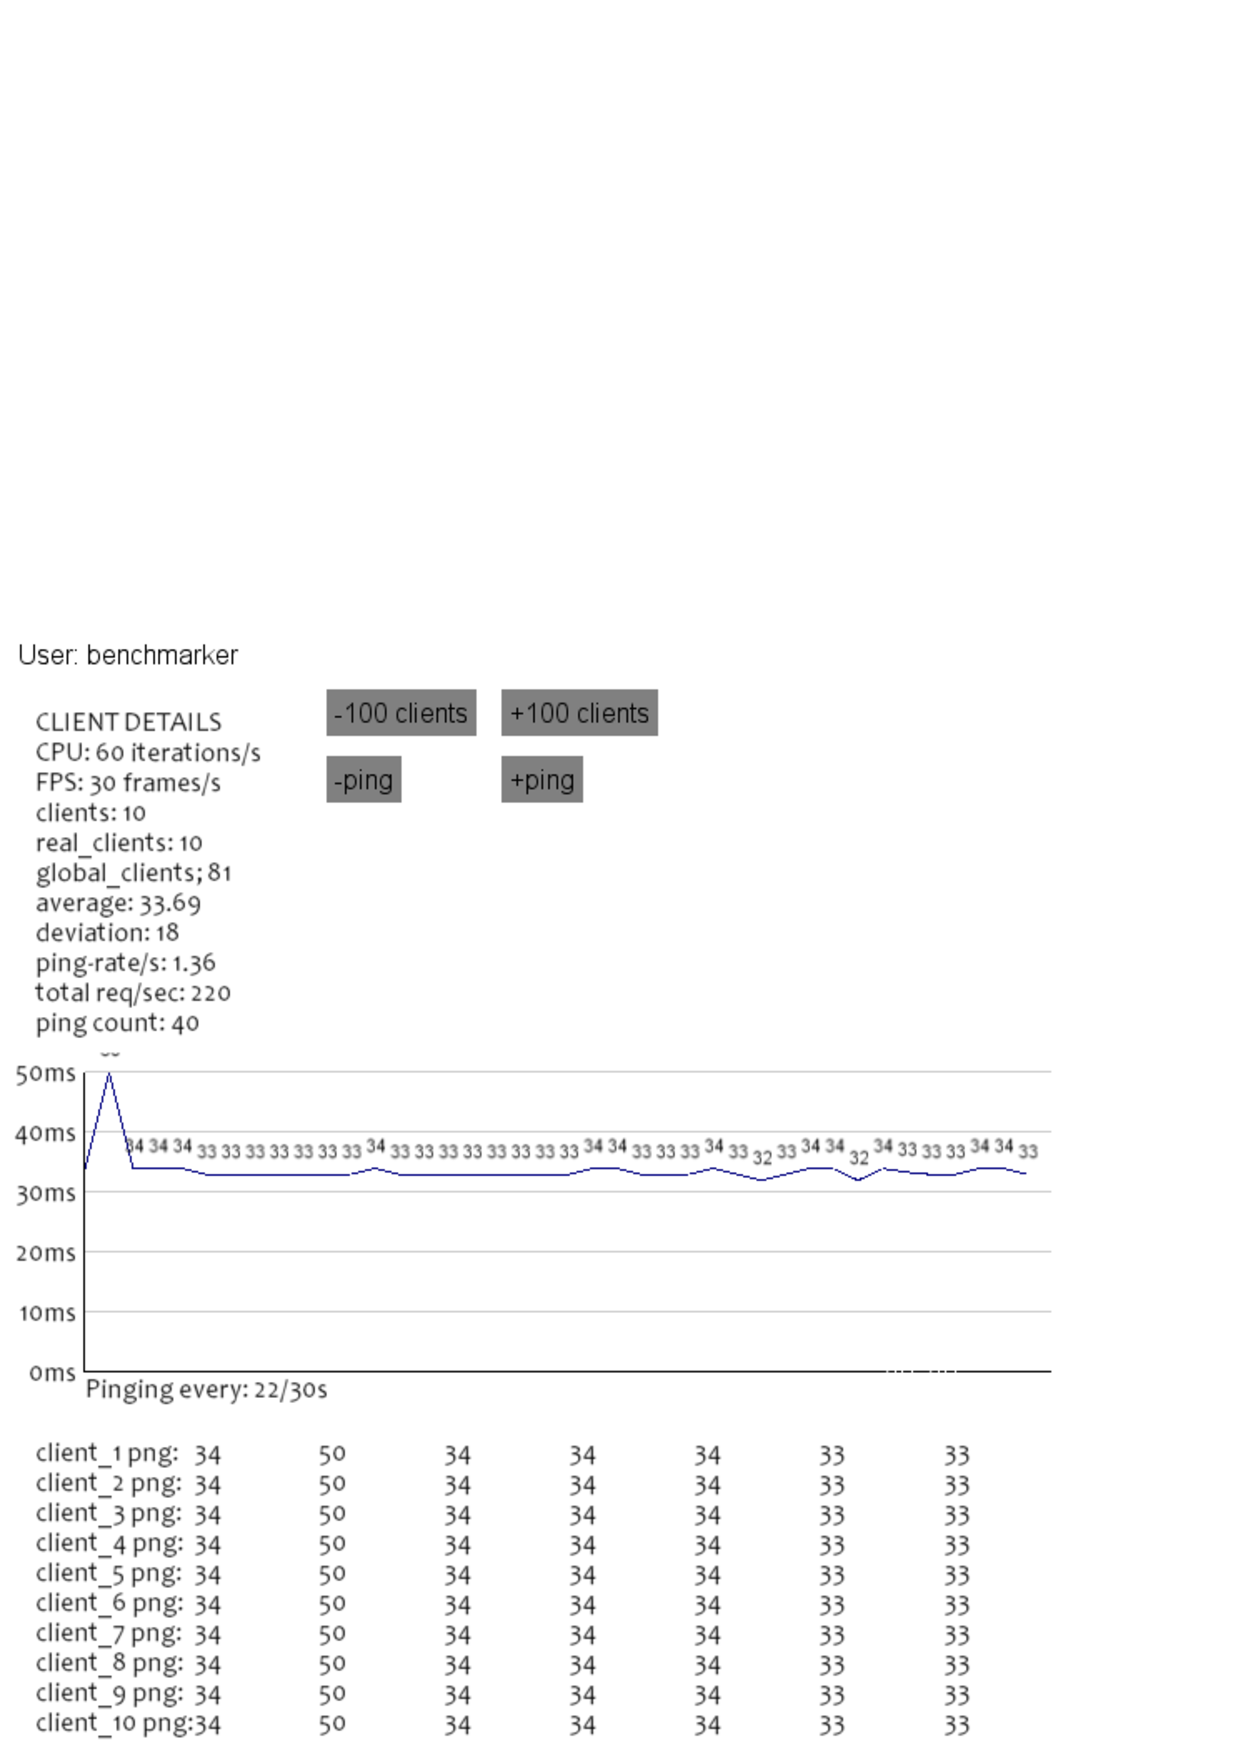
\includegraphics[scale=0.50, angle=00]{images/benchmarker.jpg}
\caption{Displaying the GUI of the benchmarking application (flipped 90 degrees). On the left top the global data is available for the client. The table on the top-right displays the virtual clients and their 5 most recent roundtrip values. The graph on the bottom displays the average RTT over time for these clients. The colors of the image are inverted from the actual interface and the font size is slightly modified to enhance readability on paper.}
\label{fig:benchmark_gui}
\vspace{1em}
\end{figure}




% -----------------------
\chapter{Network Extension Evaluation}
%description of experiments, presentation + (directly including) interpretation of the data
In this chapter, the extension is evaluated in terms of fairness and performance. More specifically, we test how concurrent connections impact the server performance in terms of CPU usage, CPU processing time and Resident Set Size (RSS). We then observe how the server performs and scales based on client interactions, discover how broadcasting messages\footnote{as opposed to one-to-one interaction} does not affect the roundtrip time of messages, and that although large distances do affect the roundtrip time, countries located within Europe maintain a roundtrip time well within the acceptable 100 milliseconds.

\section{Controlled Network}
Controlled experiments were conducted in order allow making predictions of server behaviour when loaded under similar pressure in future occasions.

These experiments were executed on a Windows 7 64-bit platform with 12.6GB available physical memory and an Intel(R) Core(TM) i7-2600K CPU @ 3.40GHz processor. The software entailed Node v0.12.3 and Socket.io v1.3.7 in order to handle the networking operations.

The network was controlled using Dummynet, using a below-average UK household network bandwidth \cite{household_bandwidth}. This involves an upload speed of 5Mbit/s, and a download speed of 1Mbit/, although no packet loss was set in order to ensure consistency throughout the controlled network experiments.

\subsection{Concurrent Connections}
It is important to know how many clients a server can host simultaneously and how well it scales before it runs out of resources such as memory and processing power. The following experiments evaluate the server performance in terms of server CPU usage, CPU time and RSS with regard to the number of concurrently connected clients.

\paragraph*{The setup} includes a variable number of concurrent connections consisting of up to 15 physical instances with each simulating at most 500 clients. These clients  do not contact the server after establishing a connection. The resulting values are averaged over 2-minute run duration periods, and each after 2-minute period the experiment restarts, having the number of clients that attempt to connect simultaneously increased by 100.

\begin{figure}[H]
\centering
% \centering% default with `floatrow`
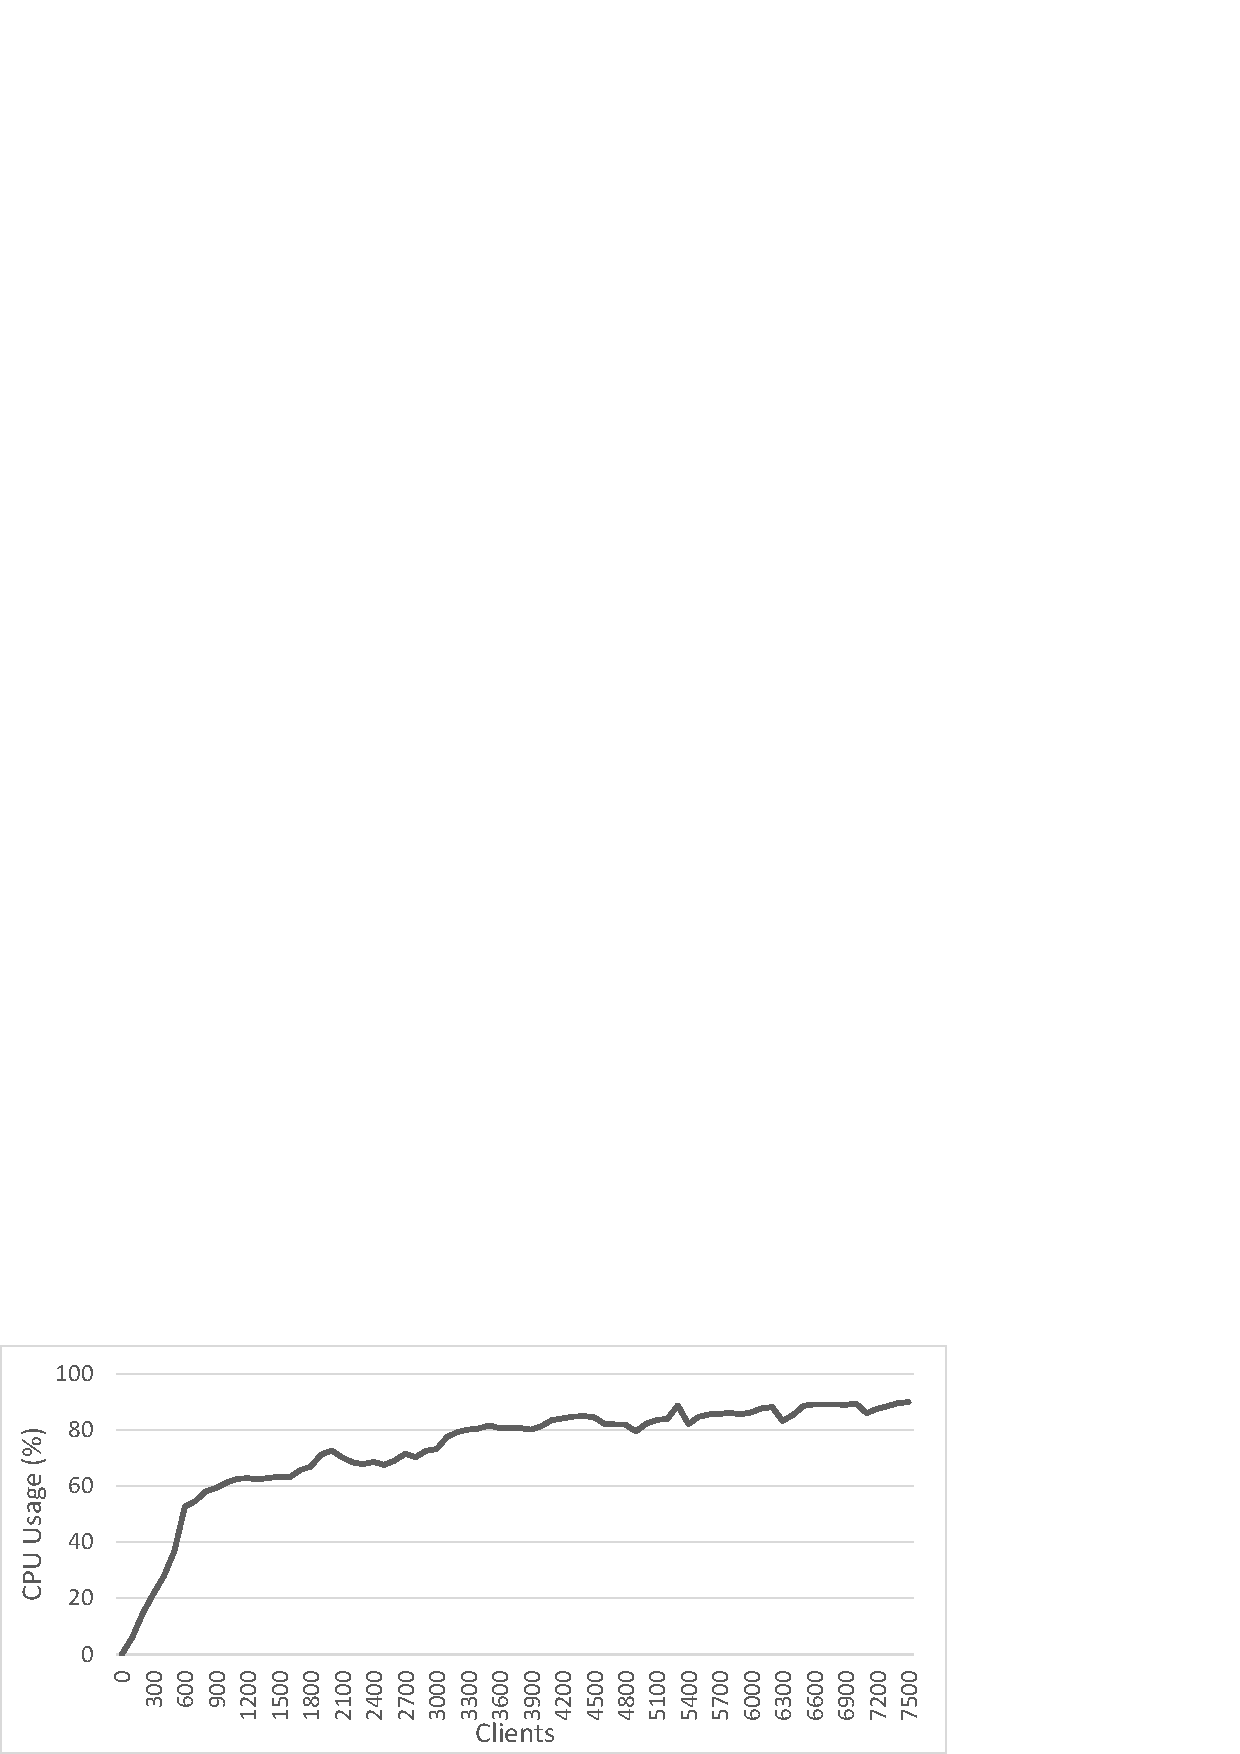
\includegraphics[scale=0.5]{images/test_CLIENT_CPUusage.jpg}
\caption{Displaying the CPU usage for the server process handling a variable number of client connection attempts in percent.}
\label{fig:cpu_usage}
\vspace{1em}
\end{figure}

\begin{figure}[H]
\centering
% \centering% default with `floatrow`
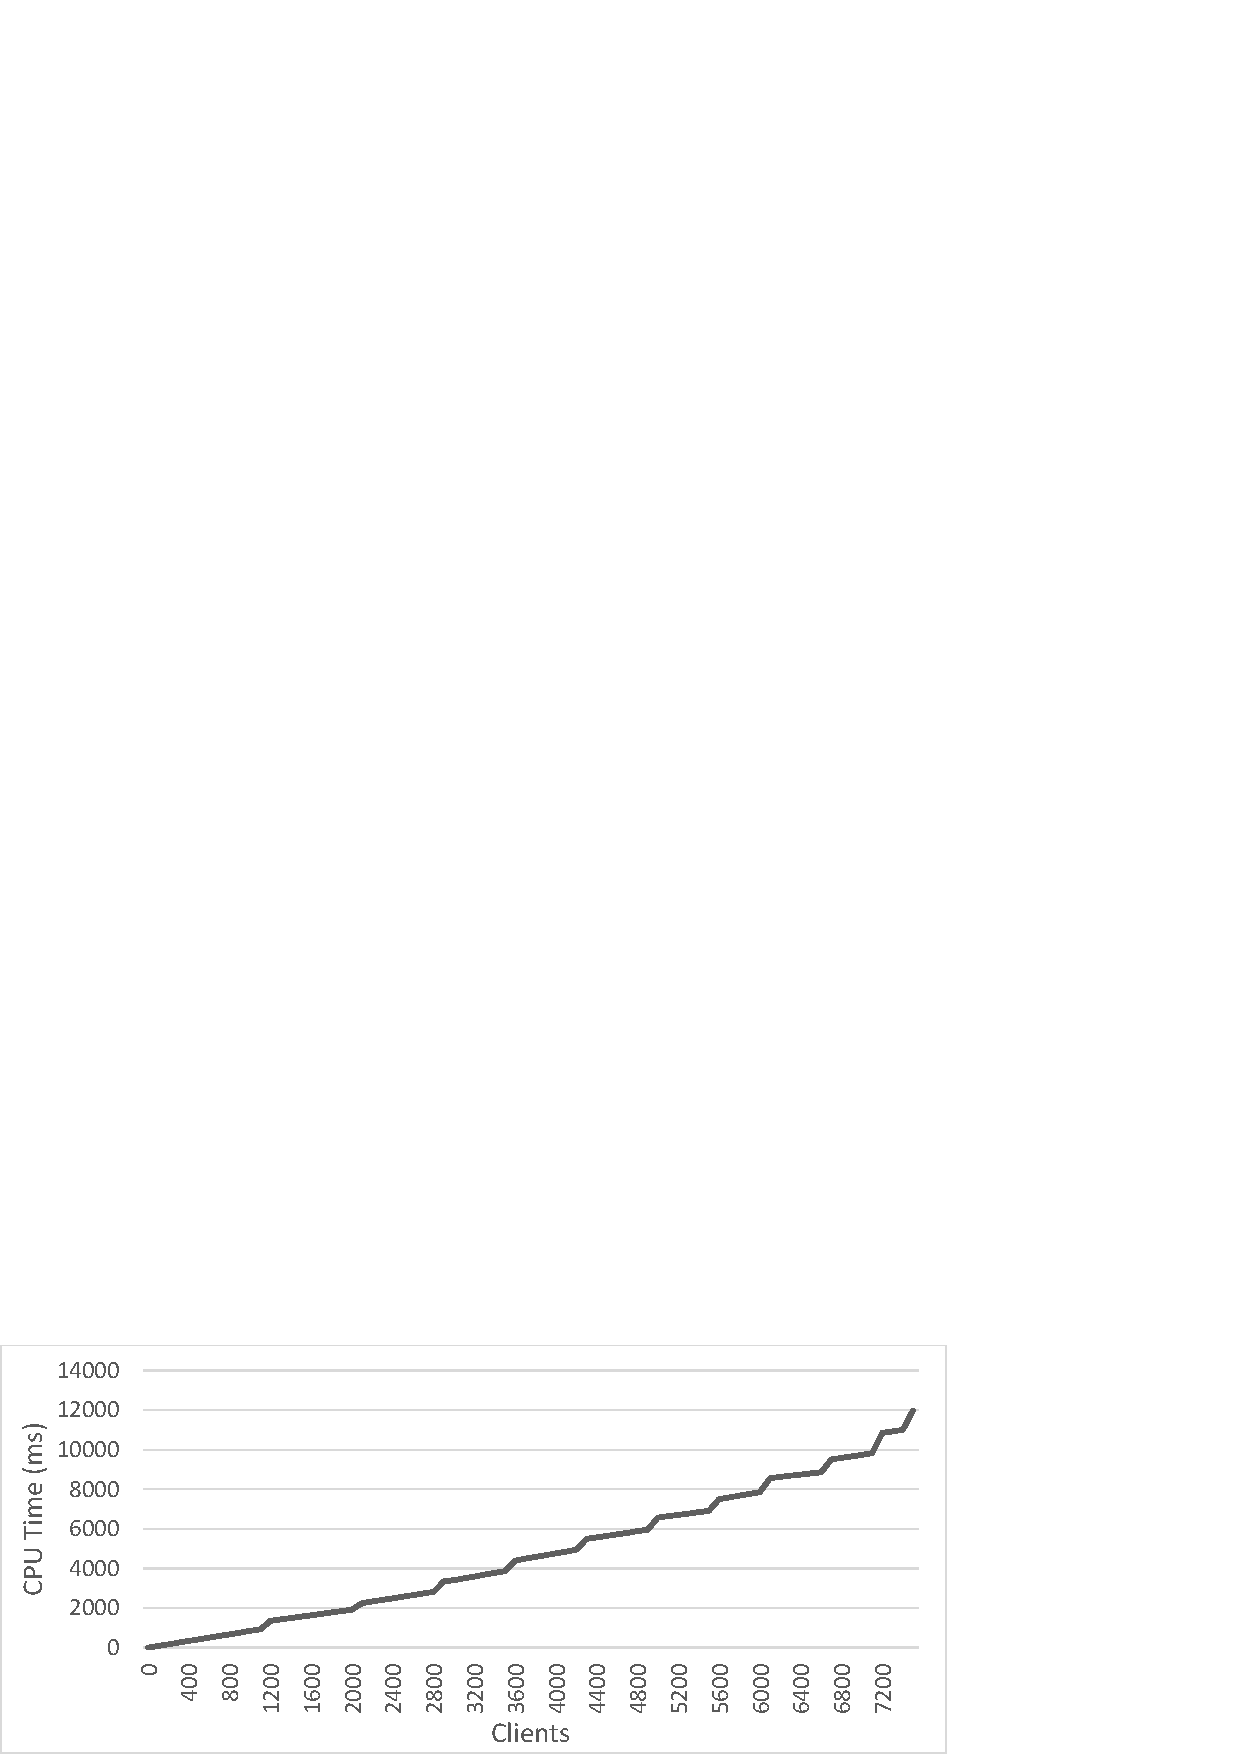
\includegraphics[scale=0.5]{images/test_CLIENT_CPUtime.jpg}
\caption{CPU time in milliseconds, displaying the amount of time required for the server to process the connection requests of all clients.}
\label{fig:cpu_time}
\end{figure}

\begin{figure}[H]
\centering
% \centering% default with `floatrow`
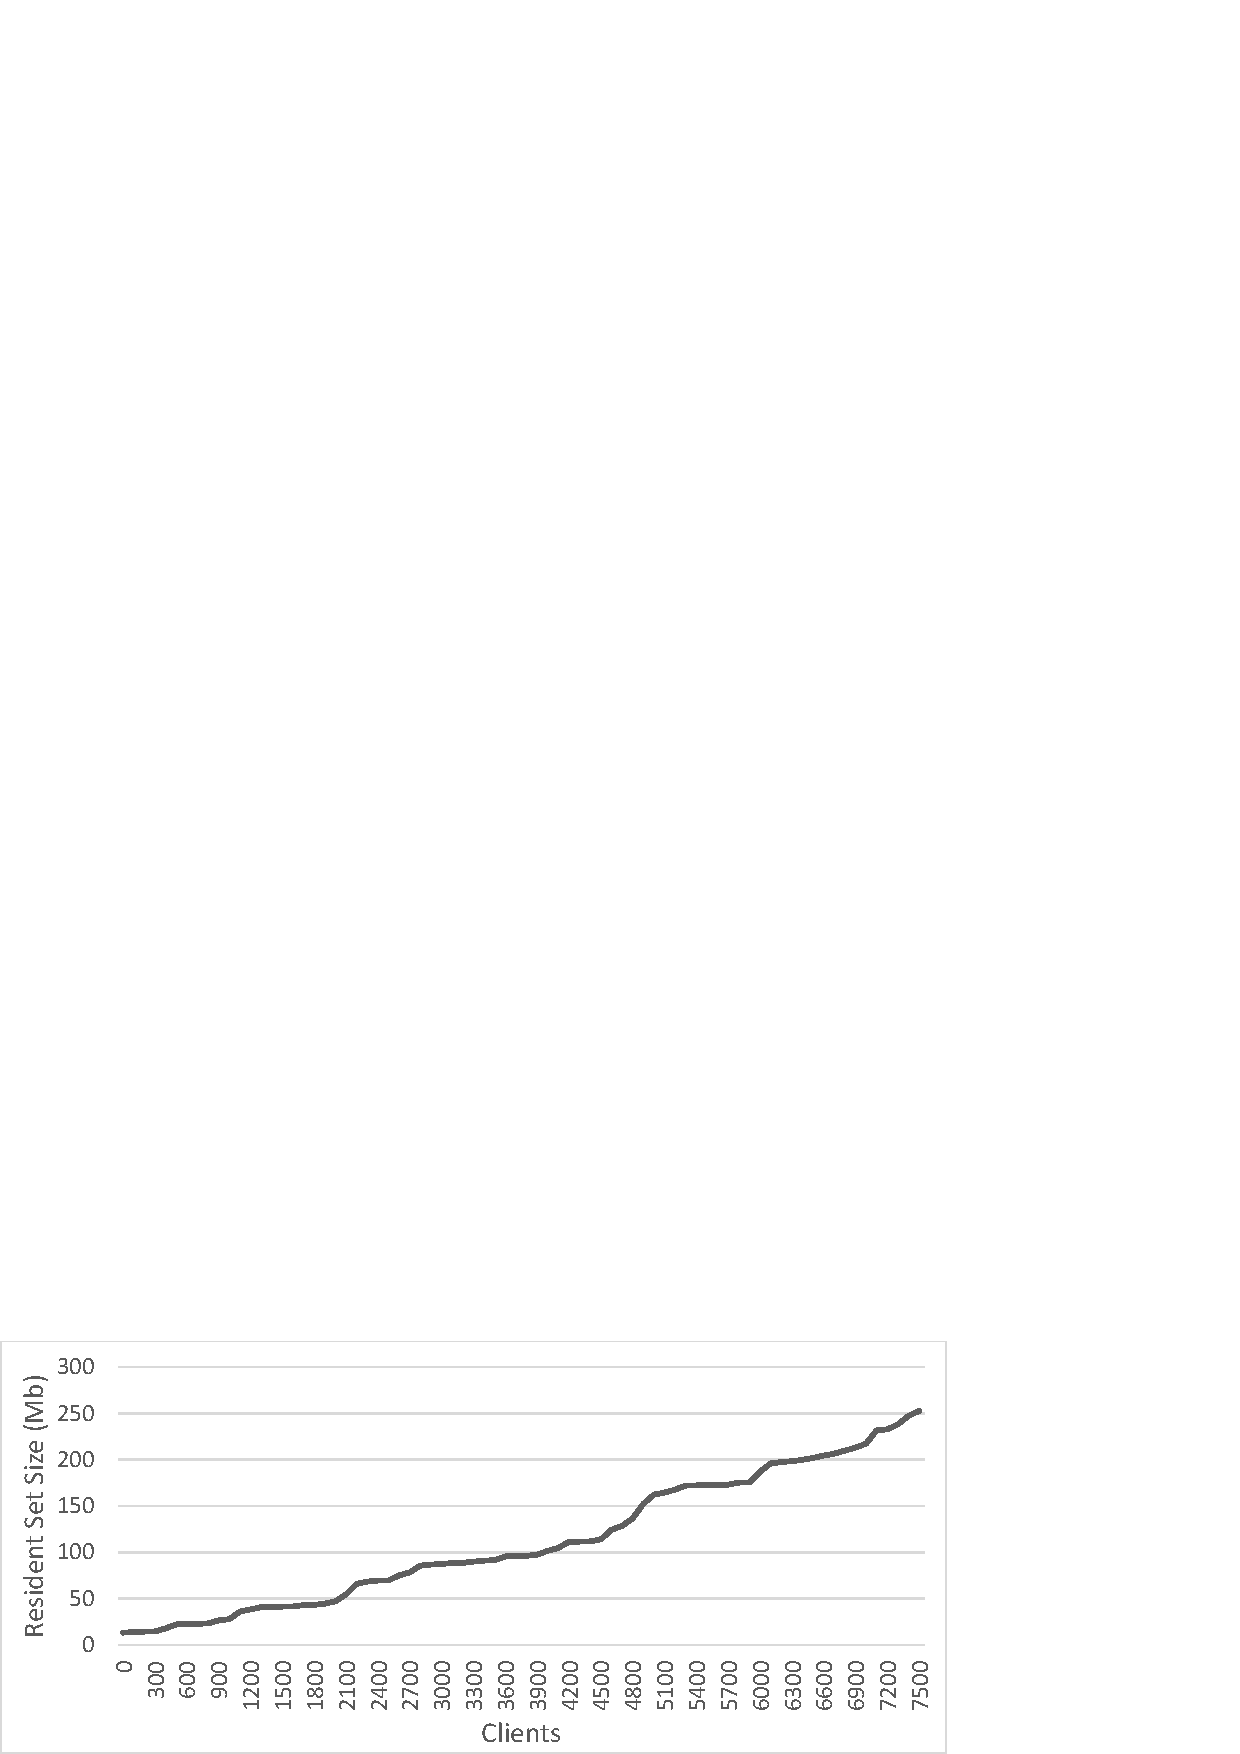
\includegraphics[scale=0.5]{images/test_CLIENT_RSS.jpg}
\caption{Resident set size in Megabit, showing the portion of RAM that is occupied by the server process.}
\label{fig:cpu_rss}
\end{figure}

Figure \ref{fig:cpu_usage} indicates a logarithmic trend in the CPU usage on the server. This seems strange. Although this effect is explained by looking at the CPU time in Figure \ref{fig:cpu_time}. 

The system aims to run the process at an optimal CPU usage amount, which can be noticed by the sudden change at a CPU usage of roughly 60\%. As soon as the server processor reaches this point, it will attempt to balance the usage by allowing more processing time for connecting the clients. The connection request processing time scales in a near-linear fashion, indicating clients to be connected one at a time. Occasional peaks and the slight increase in the trend of the CPU time may indicate the processor demanding extra time to process the increased number of connecting clients.

Due to the connection handling mechanism of Node.js, where each new client connection is offloaded to a heap using constant memory space, the RSS scales up in an almost linear fashion. This property makes it easy to predict the amount of memory required for a certain expected load. For example, in the observed scenario, each client uses roughly 5KB. Therefore when expecting 10,000 clients to connect to the server, they will be using up around 50MB (slightly higher due to the trend not being exactly linear). Similar experiments have found similar behaviour, where 16GB is consumed to record a total of 1 million concurrent connections \cite{modejs_1m_connections}.


\subsection{Message Broadcasting Performance}
The concurrent connections experiments have indicated that the system scales well within the expected demands of an average multiplayer game in terms of client concurrency. The following experiment evaluates what happens when these clients start interacting. It observes the number of messages that can be handled by the server simultaneously, and considers how this affects the fairness in response-time of the individual clients.

\paragraph*{The setup}involves up to 5000 concurrently connected clients (10 physical instances simulating at most 500 clients each) all located within the same network. Clients can send 8-Byte packets, and each client sends these packets at regular time intervals. Each client measures the roundtrip time of the packet, and for each interval these roundtrip times are averaged.

The values in Figure \ref{fig:mean_rtt} were generated by modifying the rate at which each client transmits messages to the server (a sending higher rate resulting in more incoming messages per second at the server), for a fixed number of clients: 50, 100, 500, 1000, 2500 and 5000.

Each time when the average RTT exceeds 200ms, the experiment is stopped. Beyond this point, the server appears to receive messages faster than it can handle, causing it to temporarily store the messages in a queue for later. However as clients keep sending packets at the same constant rate, resulting in a vicious cycle that causes the memory to eventually overflow.

\begin{figure}[H]
\centering
% \centering% default with `floatrow`
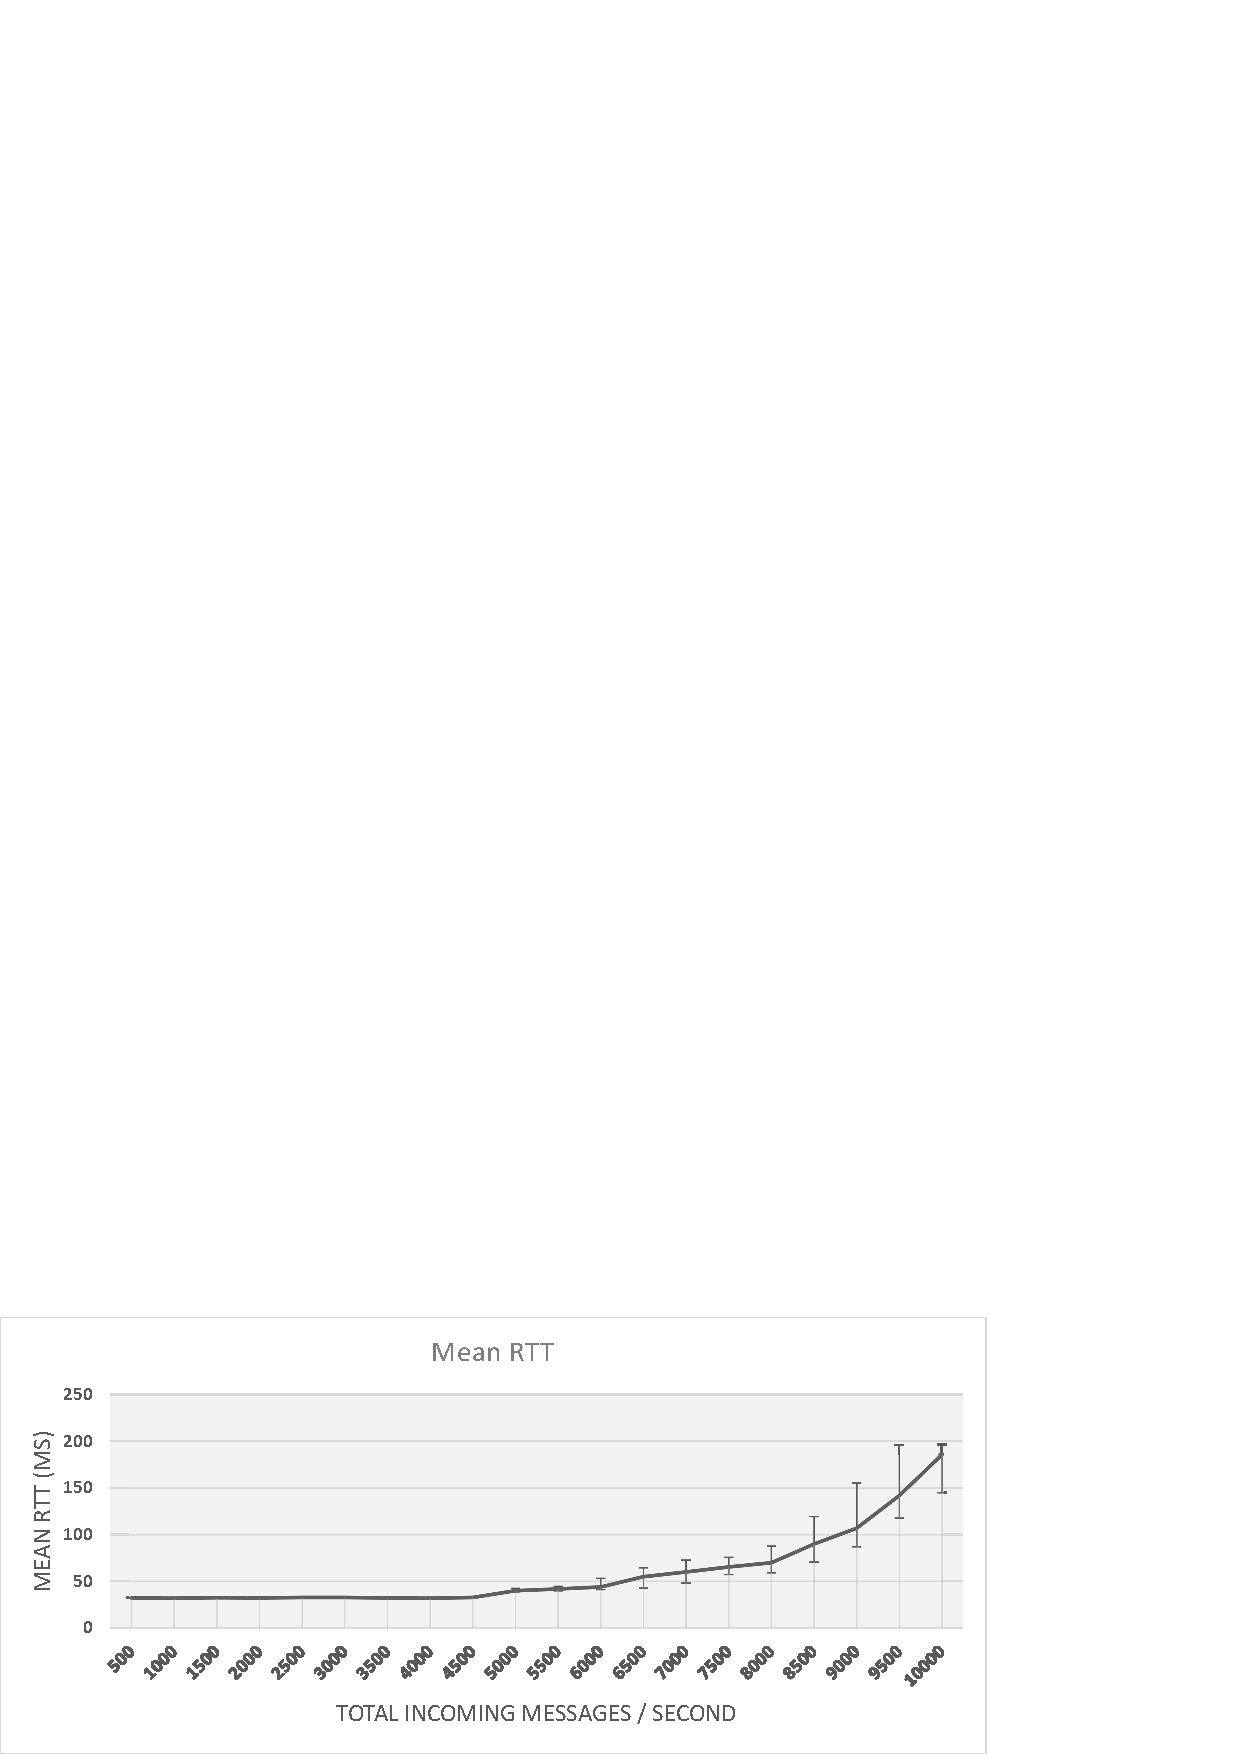
\includegraphics[scale=0.46]{images/mean_rtt.jpg}
\caption{The general case scenario indicating the observed mean 8-byte message roundtrip time, depending on the total number of messages incoming to the server at every second.}
\label{fig:mean_rtt}
\end{figure}

From Figure \ref{fig:mean_rtt}, it can be observed that the messages maintain a stable 32ms roundtrip time until the server receives around 5000 messages per second. Beyond this point, the roundtrip time grows exponentially until it reaches >200ms, which is when the experiment is terminated.

Note that after receiving, these messages were broadcasted to all other clients. In order to further visualise the effect of broadcasting messages from each client to every other client, the mean RTT results are displayed separately in Figure \ref{fig:broadcast_rtt_mean}, as well as their corresponding standard deviation in Figure \ref{fig:broadcast_rtt_std}.

\begin{figure}[H]
\centering
% \centering% default with `floatrow`
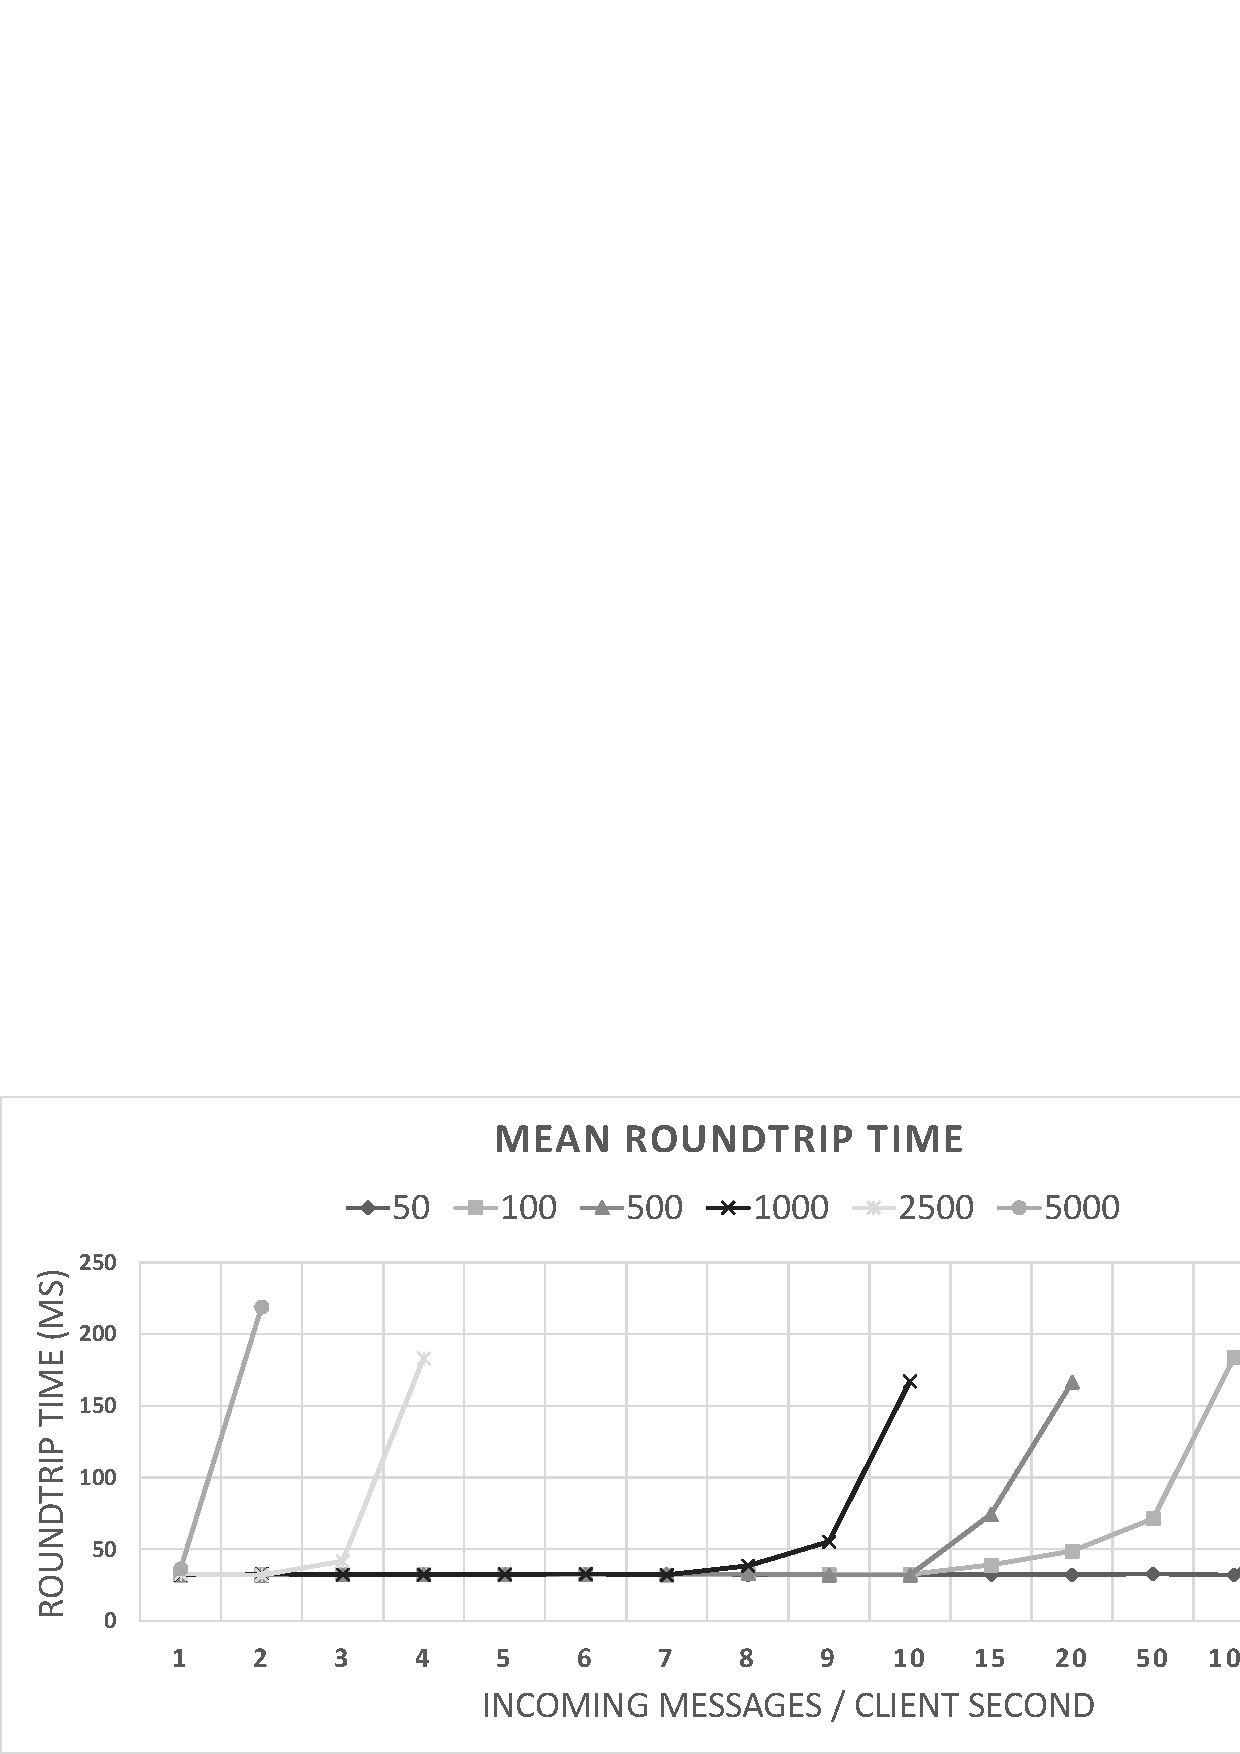
\includegraphics[scale=0.42]{images/test_SERVER_RTTmean.jpg}
\caption{The mean roundtrip time of all the messages that pass through the server, for different numbers of specified clients (50, 100, 500, 1000, 2500 and 5000). Each client sending messages at a variable rate per second.}
\label{fig:broadcast_rtt_mean}
\end{figure}

\begin{figure}[H]
\centering
% \centering% default with `floatrow`
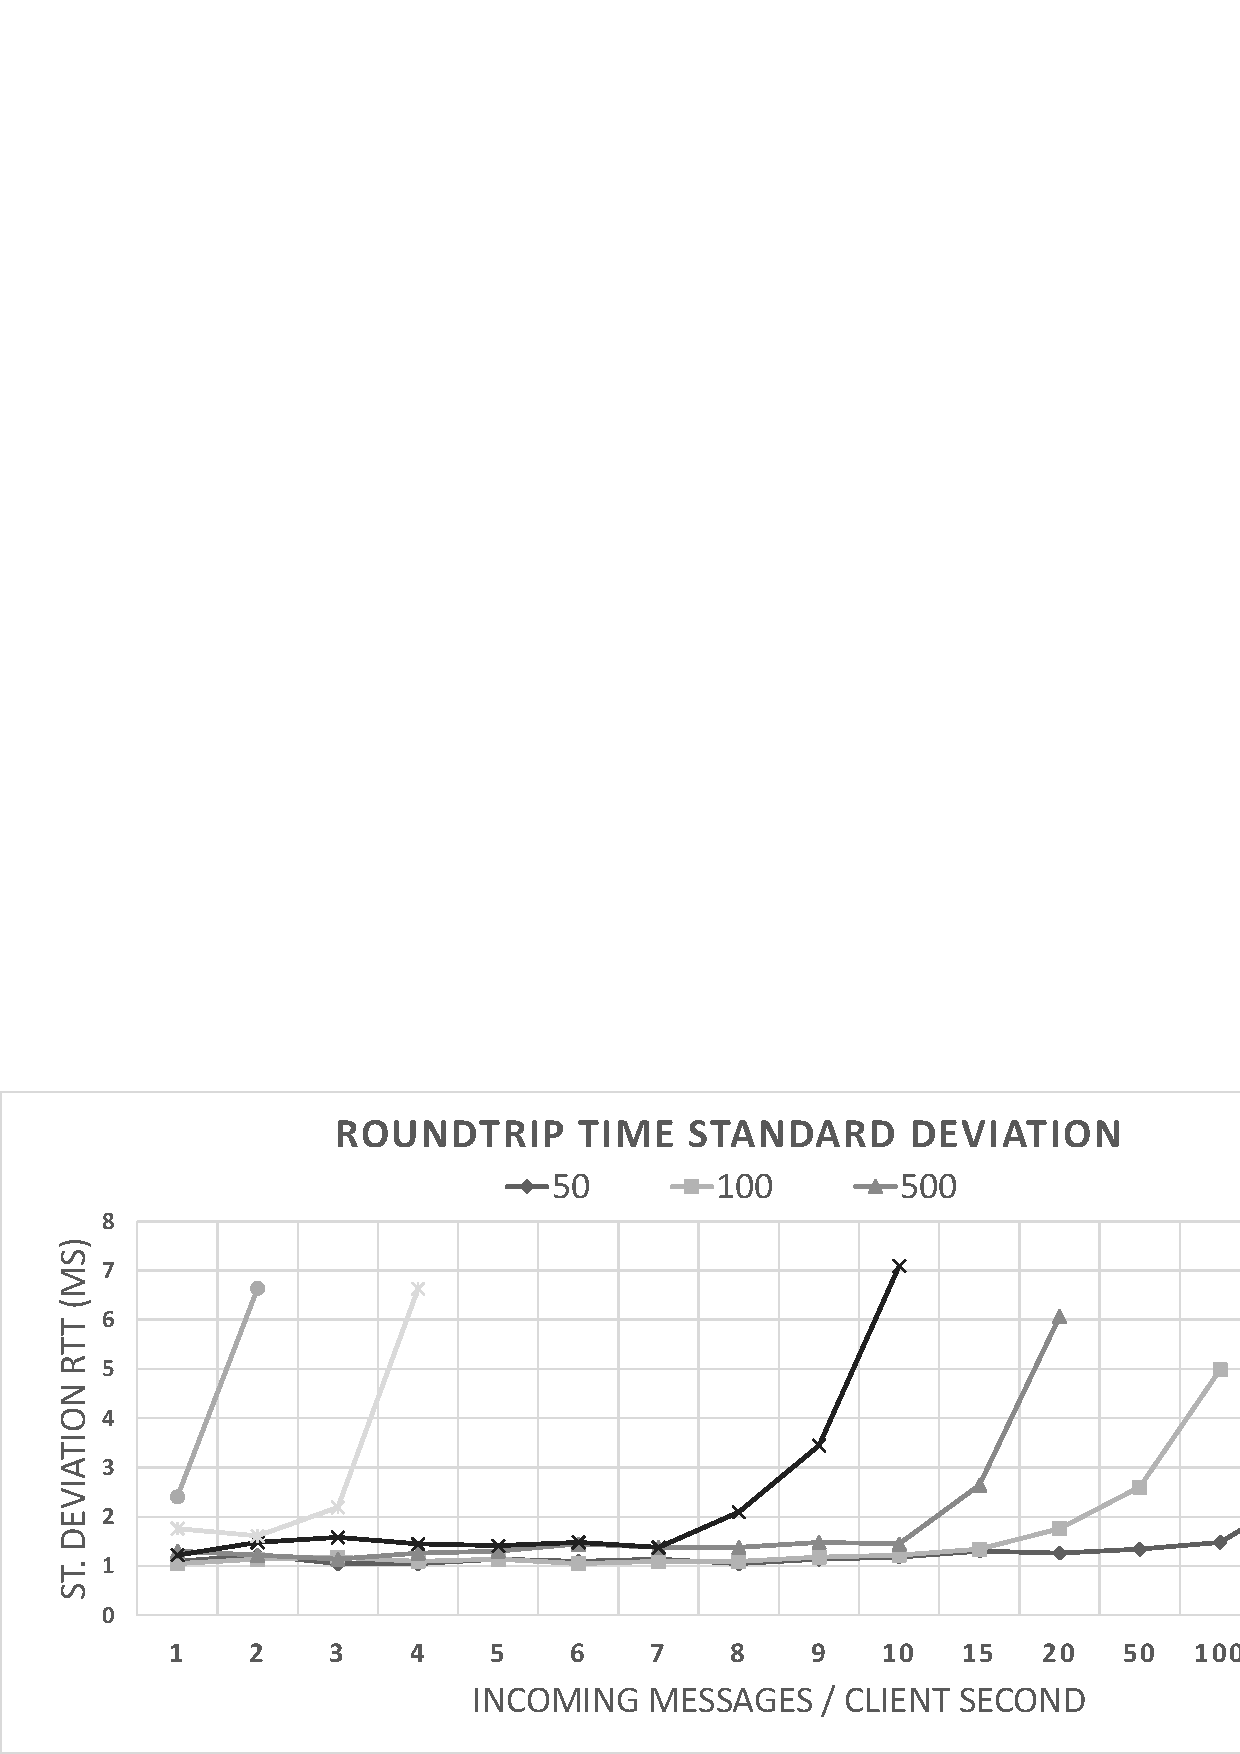
\includegraphics[scale=0.42]{images/test_SERVER_RTTstd.jpg}
\caption{The standard deviation of the message roundtrip times as displayed in Figure \ref{fig:broadcast_rtt_mean} for all messages that pass through the server, for different numbers of specified clients (50, 100, 500, 1000, 2500 and 5000). Each client sending messages at a variable rate per second.}
\label{fig:broadcast_rtt_std}
\end{figure}

The graphs in Figure \ref{fig:broadcast_rtt_mean} and Figure \ref{fig:broadcast_rtt_std} indicate as expected that with few concurrently connected clients and the same send rate per client, the server manages to broadcast many more messages (as fewer clients will be sending messages). It is important to remember that broadcasting is an intensive task with a complexity of O($n^{2}$) for n clients, as every client sends a message to every other client.

Therefore, if n = 100 clients are connected to the server, and each wants to broadcast 100 messages per second, the server receives $100 \times 100$ (= 10,000) messages per second, and has to send $100 \times 100 \times 100$ (=1,000,000) messages every second (although the sender technically does not need to re-receive its own message, this difference is negligible).

For n = 1000 clients, a maximum sending rate of 10 per second is observed. At this point the server receives $10 \times 1000$ (=10,000) messages per second, and has to send $10 \times 1000 \times 10$ (=100,000) messages per second.

These results are very interesting as they indicate that the average RTT is not necessarily affected by the number of messages the server has to send\footnote{By considering that sending 100,000 messages results in a similar average message RTT as when sending 1,000,000, given that the amount of actually handled messages remains the same}, but rather by the amount of messages the server has to receive and control in the message-handling logic.


\section{Real Network Results}
During the real network experiments, the network at the server was observed to running at a rather consistent 54Mb/s download and 3Mb/s upload speed.

\paragraph*{}Multiple tests were executed with clients located at specified locations. In each case, the clients were again sending 8-byte messages to the server, at a regular interval of 1 second for 2 minutes. The 120 roundtrip times for each client were then averaged in order to blur occasional peaks caused by inconsistencies in the network. The roundtrip times of the clients in each common location were averaged, and the deviation of the roundtrip times within the 2-minute time frame for each of these locations were calculated.

All network experiments were executed using a single server located in Edinburgh and in each experiment all clients were connected and communicating to that server simultaneously. During the experiments, in order to prevent data transmission to affect the results, logs were saved at the clients. Only after each experiment was complete, these logs were forwarded for processing purposes. The roundtrip times represent the delay times between the packet-send event in the browser client, and the packet-receive event by the same client for the same packet.

\subsection{Location-based Delay Fairness}
The following experiments evaluate the effect of the geographical distance between groups of clients and the server with respect to fairness in response-time from the server to the clients.

\paragraph*{Test cases:}
\begin{enumerate}
\item Local network setting: Five clients physically located in the same local home network.

\item Same city: Five clients physically located in Edinburgh (LAN excluded).

\item Same country: Three clients physically located in Scotland: Edinburgh, Glasgow and Dundee.

\item Europe: Six clients physically located in the United Kingdom, Hungary, France, Germany, Sweden and the Netherlands.

\item Inter-continental: Eight clients physically located in South Africa, California (USA), India, Thailand, Germany, Hungary, United Kingdom and the Netherlands.
\end{enumerate}

\begin{table}[H]
\centering
  \begin{tabular}{ | r || c | c | c | c | c |}
    \hline
    Test case 		& 1 		& 2 		& 3 		& 4 		& 5 		\\ \hline\hline
    Mean RTT 		& 32.1ms 	& 54.8ms 	& 62.7ms 	& 70.6ms 	& 107.5ms	\\ \hline
    Std RTT			& 0.4ms		& 2.9ms		& 6.8ms		& 3.36ms	& 43.6ms	\\ \hline
  \end{tabular}
  \caption{Average roundtrip times per test}
  \label{table:geo_avg_roundtrip}
\end{table}


\begin{table}[H]
\centering
  \begin{tabular}{ r | l | l }
Location		& Average RTT	& Server Distance \\ \hline\hline
LAN				& 32ms			&0km\\
Edinburgh		& 55ms			&0km\\
Dundee			& 65ms			&63km\\
Germany			& 67ms			&977km\\
Glasgow			& 68ms			&67km\\
France			& 69ms			&1165km\\
the Netherlands	& 70ms			&698km\\
Sweden			& 70ms			&1238km\\
United Kingdom	& 71ms			&66km\\
Hungary			& 76ms			&1881km\\
India			& 103ms			&7582km\\
South Africa	& 144ms			&9760km\\
California (USA)& 158ms			&8065km\\
Thailand		& 171ms			&9438km\\
  \end{tabular}
  \caption{Average roundtrip times per location, along with their overall geographical distance from the server.}
  \label{table:geo_avg_location}
\end{table}

Clients located within the local network have the fastest roundtrip time, as expected since packets can travel. After this point, Clients located anywhere within Europe have an overall roundtrip time between 55ms and 76ms. These values are reasonable depending on the purpose of the game that is created with the extension, but complicated to omit. A general rule of thumb for ping values is that anything below 100ms is acceptable, even for high-end shootergames such as Battlefield and Call of Duty, where clients may automatically get kicked when their roundtrip time exceeds 150ms or 200ms potentially disrupting the gameplay.

Table \ref{table:geo_avg_roundtrip} and table \ref{table:geo_avg_location} show the average roundtrip times observed by clients located at different locations on earth. These RTT for these locations may differ due to factors such as the connection speed, ISP quality and firewall settings. But the experiment shows that the major contributor to unfairness in the network appears to be directly affected by the distance to the server, as the average RTT for each of the locations significantly increases as the distance increases. Figure \ref{fig:worldmap} visualises the connection between the observed roundtrip times and the corresponding distance between the client and the server. 

Assuming the added delay is caused by the implied distance and packet-switching, the only real solution to the problem involves modifying the physical link between the client and the server or locating the server closer to the intended clients.

\begin{figure}
\centering
% \centering% default with `floatrow`
\includegraphics[scale=0.45]{images/worldmap.jpg}
\caption{Worldmap displaying the tested locations and their according average recorded roundtrip times}
\label{fig:worldmap}
\end{figure}





% -----------------------
\chapter{Conclusion, Discussion and Future Work}
\section{Conclusion}
The extension works, and can be implemented easily as its functionality is more simple than the native GameMaker networking features\footnote{that are supported for non-browser platforms} as it automatically takes care of specifying the transport protocol and the buffer along with its properties such as size, byte-alignment and type. Data types from the buffer are generic, matching with the weakly typed property of that of GameMaker. Using Socket.io to open and maintain a TCP connection omits the NAT traversal problem that many novice developers would otherwise experience.

The extension offers a sufficiently scalable solution when combined with the provided server implementation using Node.js and Socket.io. This is proven by the fact that the server manages to maintain few thousands of concurrent connections, and handle roughly 5000 messages per second over a long-time period before the packet round-trip time starts to visibly increase, with an accepted rate of 8500 messages per second before the round-trip time starts to exceed 100ms. 

Long-distance connections are the main contributor to unfairness, but for this issue apart from distributing multiple servers across the globe or optimizing the physical link between the endpoints, no real solution is known. With a standard server load, any distance up to a few thousand kilometers is however found to provide an acceptable average roundtrip time of less than 100ms.

Based on these experiments, developers can ensure their application performs in an optimal fashion.

\section{Discussion}
The evaluation methods indicate that the network indeed performs well enough to allow a sufficient amount of clients to connect and interact simultaneously without impacting a server with average-performing hardware requirements, proving that the extension is indeed useful.
However, proving that the extension is indeed usable to novice developers is a rather more subjective issue. Although the primary focus was to simplify the development process for other developers, this was approached by following the best "software engineering practices", enforcing the right quality attributes on each module of the implementation. A novice or even average browser game developer may not know about these practices. Therefore it would be fair to further evaluate the usability by inviting developers to try out the extension.
The time required to receiving accurate measurements forced this evaluation to be discontinued for this thesis project.

\section{Future Improvements}
Collecting feedback for a usability evaluation could indicate possible improvements in terms of simplifying the use of the extention to develop new networked browser games and applications.

Delay in roundtrip times can be masked at the application level (either in the extension or in the client directly) by predicting future values based on recent value changes in the past.

It may be possible to optimize the network performance by using WebRTC to interact with the server. However this would only be beneficial GameMaker developers if also packet-losses and NAT traversal are resolved by the extension, and would not fix the increase in RTT caused by distance.

Fixing the distance issue can be done by spreading servers across the world, and connecting clients to the server that provides the lowest roundtrip time. This, however forces multiple versions of the game state to coexist, thereby causing the issue where servers need to interact with each other in order to keep their versions of the game state synchronized.





% -----------------------
% >>>> REMOVE THIS BLOCK
%Quick list of provided references...\\
%proper citations\\
%\cite{Multiplayer_Networking_modern_engine}
%\cite{Fairness_and_Playability}
%\cite{Pro_HTML5_Programming}
%\cite{HTML5_Up_and_Running}
%\cite{Friendly_Programming} %unused
%\cite{Mark_Overmars}
%\cite{Death_Flash_Java}
%\cite{Why_Nodejs}
%\cite{Node_Stress_Test}
%\cite{NodeJS_Image}
%\cite{Socketio_Benchmark}
%\cite{Socketio_TCP_Benchmark}
%\cite{Socketio}
%\cite{Canvas_API}
%\cite{Web_Apps_Superior}
%\cite{Why_MMOG} %unused
%\cite{Browser_Games}
%\cite{Browser_Networking}
%\cite{Web_Apps_Superior}
%\cite{P2P_Video_Streaming_HTML5_WebRTC}
%\cite{Gamemaker_DnD}
%\cite{GameMaker_Studio}
%\cite{Optimizing_Multiplayer_3D_Game_Synch} %unused
%\cite{Optimizing_WebSockets_Bandwidth} %unused
%\cite{Google_Play_Store}
%\cite{Apple_App_Store}
%\cite{HTML5_Game_Dev_Gamemaker} %unused
%\cite{SE_7_Principles}
%\cite{Software_Engineering}
%\cite{Construct2_Multiplayer_Tutorial}
%\cite{WebSocket}
%\cite{NAT}
%\cite{Where_WebRTC}

%web url referrals\\
%\cite{handshake}
%\cite{tcp_open_connection}
%\cite{udp_connectionless}
%\cite{udp_holepunching}
%\cite{websocket_communication}
%\cite{gamemaker_missing_networking}
%\cite{gamemaker_networking_attempt}
%\cite{yoyogames_forum}
%\cite{dutch_gamemaker_forum}
%\cite{html5_gamedev_tools}
%\cite{html5_mozilla}
%\cite{alexa_ranking}
%\cite{gamepix_engines}
%\cite{scirra_forum}
%\cite{construct2_multiplayer}
%\cite{unity_support}
%\cite{unity_networking}
%\cite{unity_websocket_sharp}
%\cite{unity_forum}
%\cite{unity_forum_2d}
%\cite{unity_suggests_gamemaker}
%\cite{socketiojs}
%\cite{household_bandwidth}
%\cite{unity_stats}
%\cite{quality_attributes}
%\cite{modejs_1m_connections}
% <<<< REMOVE THIS BLOCK

%TODO change style to apa before submission. ignore "errors", it should still work after a few retries
\bibliographystyle{unsrt}
\bibliography{mybibfile}


\end{document}
